\documentclass[a4paper,12pt]{article}

\author{hidebon9105 }
\date{December 2019}
%\documentclass[conference]{IEEEtran}
%\usepackage[T1]{fontenc} % optional
\usepackage{amsmath}
%\usepackage[cmintegrals]{newtxmath}
%\usepackage{bm} % optional
\usepackage{cite}
%\usepackage[dvipdfmx]{graphicx}
\usepackage{graphicx}
\usepackage{color}
\usepackage{lscape}
\usepackage{bm}
%\ifCLASSINFOpdf
%\else
%\fi

%\hyphenation{op-tical net-works semi-conduc-tor}


\begin{document}
\begin{center}
\vspace*{20truept}
{\large MASTER THESIS} \\
\vspace{260truept}

Hiroshima University \\
Faculty of Engineering\\
\vspace{30truept}
{\Large Hideki Oki}\\
\vspace{30truept}
March 2018
\end{center}
\thispagestyle{empty}

\newpage

\begin{titlepage}
\title{Metric Learning}


\begin{center}
\vspace*{20truept}
{\large MASTER THESIS} \\
\vspace{30truept}
{\bf \Large Applications of Deep Metric Learning for Classification and Distillation}

\vspace*{30truept}
\begin{tabular}{rllrl}
Supervisor & Professor & Takio Kurita \\
Sub Supervisor & Associate Professor & Jyunichi Miyao \\
Sub Supervisor & Associate Professor & Toru Tamaki
\end{tabular}
\vspace{100truept}

Hiroshima University \\
Faculty of Engineering\\
Department of Information Engineering\\
\vspace{35truept}
{\Large M181021 Hideki Oki} \\

\vspace{35truept}

A thesis submitted for the degree of bachelor at February 2018



\end{center}

\author{M181021 Hideki Oki \\
Hiroshima University \\
Faculty of Engineering\\
Department of Information Engineering}
\date{February 2020}

\end{titlepage}
\thispagestyle{empty}
\clearpage
\begin{abstract}

\end{abstract}
\newpage
\thispagestyle{empty}
\section*{Acknowledgements}


\newpage
\thispagestyle{empty}
\tableofcontents
\clearpage
\setcounter{page}{1}
\section{Introduction}
Today, machine learning is used in a very wide range of fields, such as image recognition, voice recognition, and abnormality detection.
Machine learning provides optimal solutions through large amounts of sample.
Machine learning includes algorithms such as $k$-nearest neighbor (kNN) \cite{Cover1967} and Support Vector Machines (SVM) \cite{Cortes1995}.
These methods search for the best identification result in the space of the original sample.
On the other hand, datasets can be converted from the original space to the new space.
Techniques such as Principal Component Analysis (PCA) \cite{Pearson1901} and Linear Discriminant Analysis (LDA) \cite{Fisher1936} are methods that project sample into a new space.
By projecting the data into a new space, for example, the number of dimensions of the sample can be reduced at the time of identification, or the characteristics of the sample can be arranged.

Metric learning is a machine learning approach based on the distance between samples.
Metric learning aims at reducing the distance between similar objects and increasing the distance between different objects.
It can be said that kNN for identifying a sample based on the distance information of the sample is a kind of metric learning.
Metric learning has various uses because of its characteristics.
Because of the characteristic that the distance between similar objects is small, it is used for abnormality detection, face verification, image search, and the like.

Meanwhile, a deep neural network model such as deep Convolutional Neural Network (CNN) has been widely used in the field of pattern recognition since deep CNN proposed by Krizhevsky et al. \cite{Krizhevsky2012} won the ILSVRC 2012 with higher recognition accuracy than the conventional methods.
Along with that, the concept of metric learning has also been introduced to deep learning.
Bromely et al. \cite{Bromely1994,Chopra2005,Hadsell2006} proposed the Siamese Neural Network as a deep metric learning model.
Siamese Neural Network is a deep learning model that performs pairwise learning.
Siamese Neural Network learns embedding that minimizes the distance between similar samples.
Siamese Neural Network also learns embedding to maximize the distance between dissimilar samples.
However, since the Siamese Neural Network was a pair-wise learning model, it was necessary to uniquely determine the concept of similarity.
However, since the Siamese Neural Network was a pair-wise learning model, it was necessary to uniquely determine the concept of similarity.
To address this issue, Wang et al. \cite{Wang2014}, Hoffer et al. \cite{Hoffer2015} proposed the Triplet Network, an extension of the Siamese Network to triplet-wise.
The triplet network takes a triplet of "anchor", "positive", and "negative" as input.
The triplet network learns so that the anchor-positive distance is relatively closer than the anchor-negative distance.
Therefore, multiple similar concepts can be considered without depending on one similar concept.
Triplet Network overcomes the drawbacks of Siamese Network.

Metric learning learns embedding as a cluster for each object.
That is, the dataset can be converted into embedding arranged for each object.
This may provide a good embedding space for the classifier for various tasks.
Therefore, we try to apply the concept of metric learning to various tasks.

First, we propose to apply metric learning to the optimization problem of ROC curves in binary classification.
We propose that the classifier learn embedding that learned similarity and dissimilarity of objects by Siamese Network.
As a result, in the evaluation area under the ROC curve (AUC), we succeeded in obtaining higher performance than the conventional classifier.
We also propose an extended method for multi-class classification.
In the case of multi-class as well, we succeeded in obtaining higher performance than conventional classifier.

Second, we propose to introduce metric learning concept  into  knowledge  distillation.
Knowledge distillation is a technique for transferring knowledge of deep or ensemble models with many parameters (teacher model) to smaller shallow models (student model).
Generally, the student model is optimized so as to eliminate the difference between the output of the student model and the output of the teacher model.
The  functionality  of  the metric  learning  to  reduce  the  differences  between  similar outputs  can  be  used  for  the  knowledge  distillation  to  reduce the differences between the outputs of the teacher model and the  student  model.  
Since  the  outputs  of  the  teacher  model for  different  objects  are  usually  different,  the  student  model needs  to  distinguish  them.  
We  think  that  metric  learning  can clarify  the  difference  between  the  different  outputs,  and  the performance of the student model could be improved.
The effectiveness of the proposed approach is experimentally confirmed for image classification tasks.
The results show that the student model obtained by the proposed method gives higher performance than the conventional knowledge distillation methods.

The following sections describe these attempts.
\section{Related Works}
\subsection{multi layer perceptron}
\begin{figure}[ht]
\begin{center}
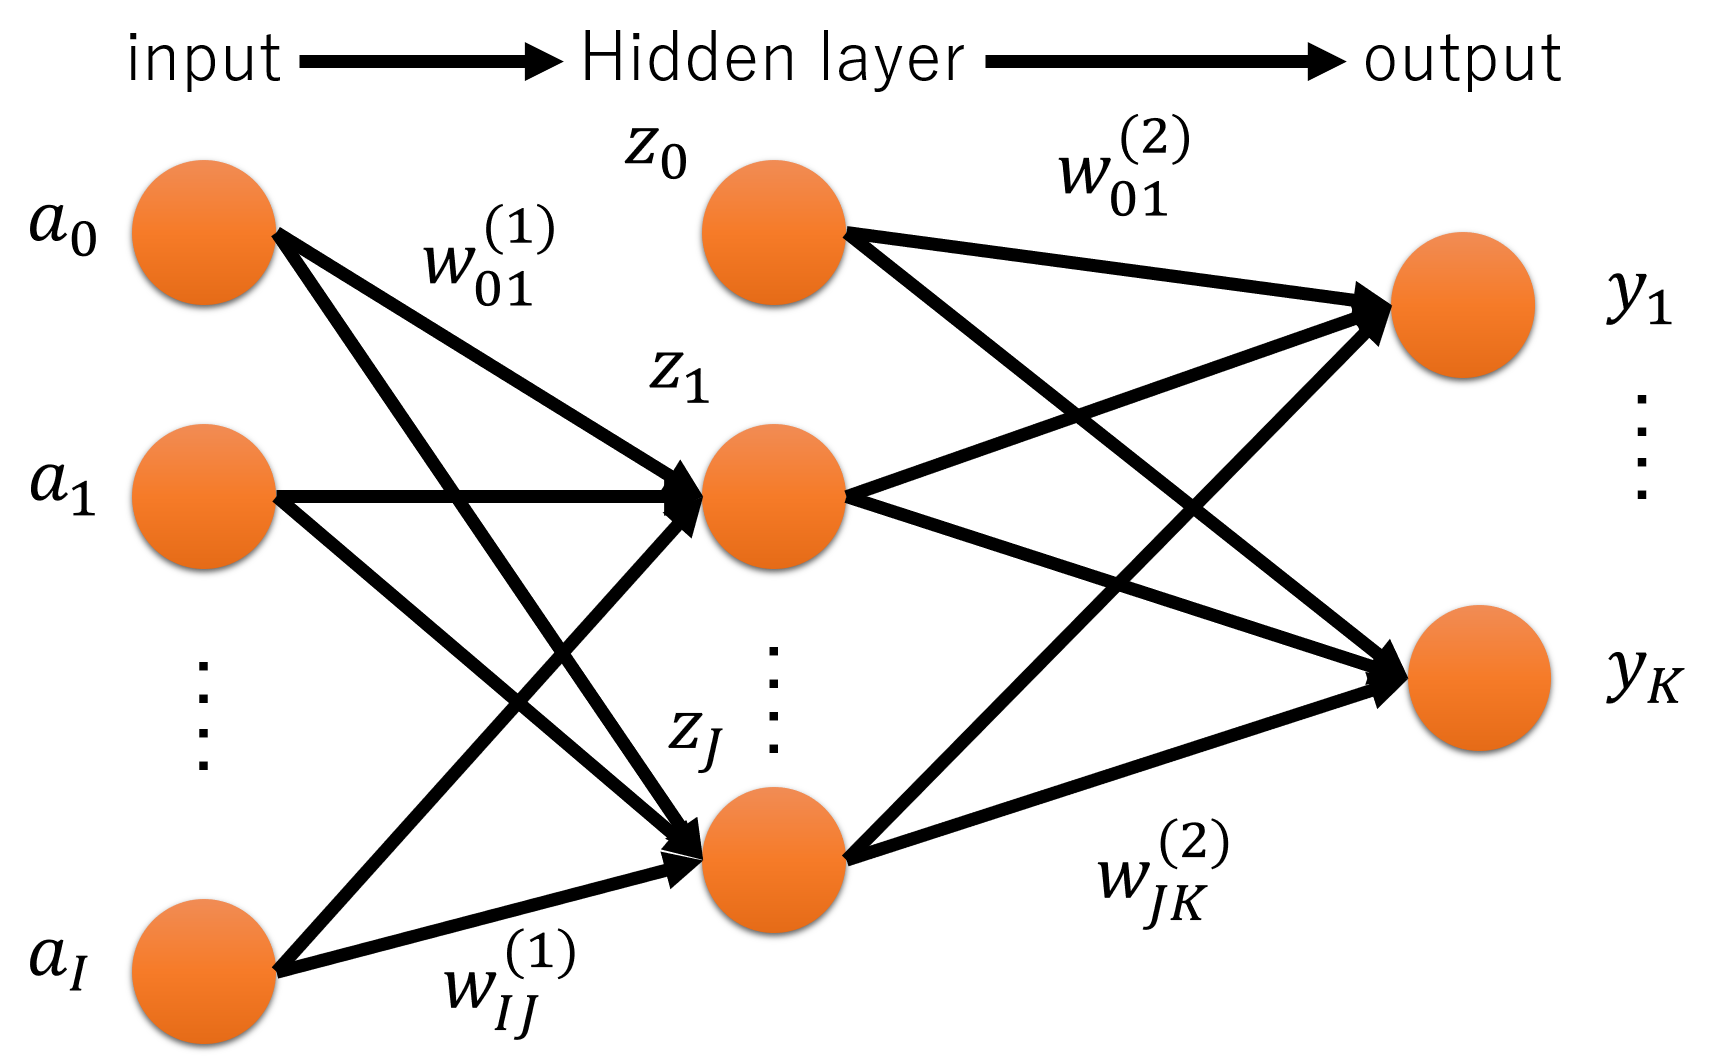
\includegraphics[scale=0.5]{figure4.png}
\caption{multi layer perceptron}
\end{center}
\end{figure}
Multi layer perceptron, one type of neural network, was proposed by Rosenblatt et al.\cite{Rosenblatt1958}. It is the model of information processing for the pattern recognition which is inspired by brain’s cognitive function. It has the ability to solve the nonlinear problem. \par
That is, the input unit$(a_1, a_2, \cdots, a_I)$, the middle unit$(z_1, z_2, \cdots, z_J)$, and the output unit$(y_1, y_2, \cdots, y_K)$ are connected by weighted connection respectively. Here, $w^{(l)}_{ij}$ is a weight connecting the $l$-th layer unit and $l+1$-th layer unit. \par
In the case of the structure in the above figure, the hidden layer $z_j$ receives the output $a_i$ of the previous layer and the weight $w^{(1)}_{ij}$ as
\begin{align}
z_j=h(\sum_{i=1}^I{w_{ij}^{(1)}}a_i+a_0)
\end{align}
Where $x_0$ is the bias. $h(x)$ is called an activation function, and generally a Relu function is used.(Equation (\ref{activation}))
\begin{eqnarray} \label{activation}
h(x)=\left\{
\begin{array}{ll}
0 & (x<0) \\
x & (x \geq 0)
\end{array}
\right.
\end{eqnarray} \par
In the same way, the output layer $y_k$ receives the output from the previous layer $z_j$ and the weight $w^{(2)}_{jk}$ as
\begin{align}
y_k=h(\sum^J_{j=1}{z_j w_{jk}^{(2)}}+z_0)
\end{align}
For simplicity, it is assumed that the activation function in the hidden layer is Relu, and only the case of $z_j \geq 0$ is considered here,
\begin{align}
z_j&=\sum_{i=1}^I{w_{ij}^{(1)}}a_i+a_0 \\
\end{align} \par
\begin{figure}[ht]
\begin{center}
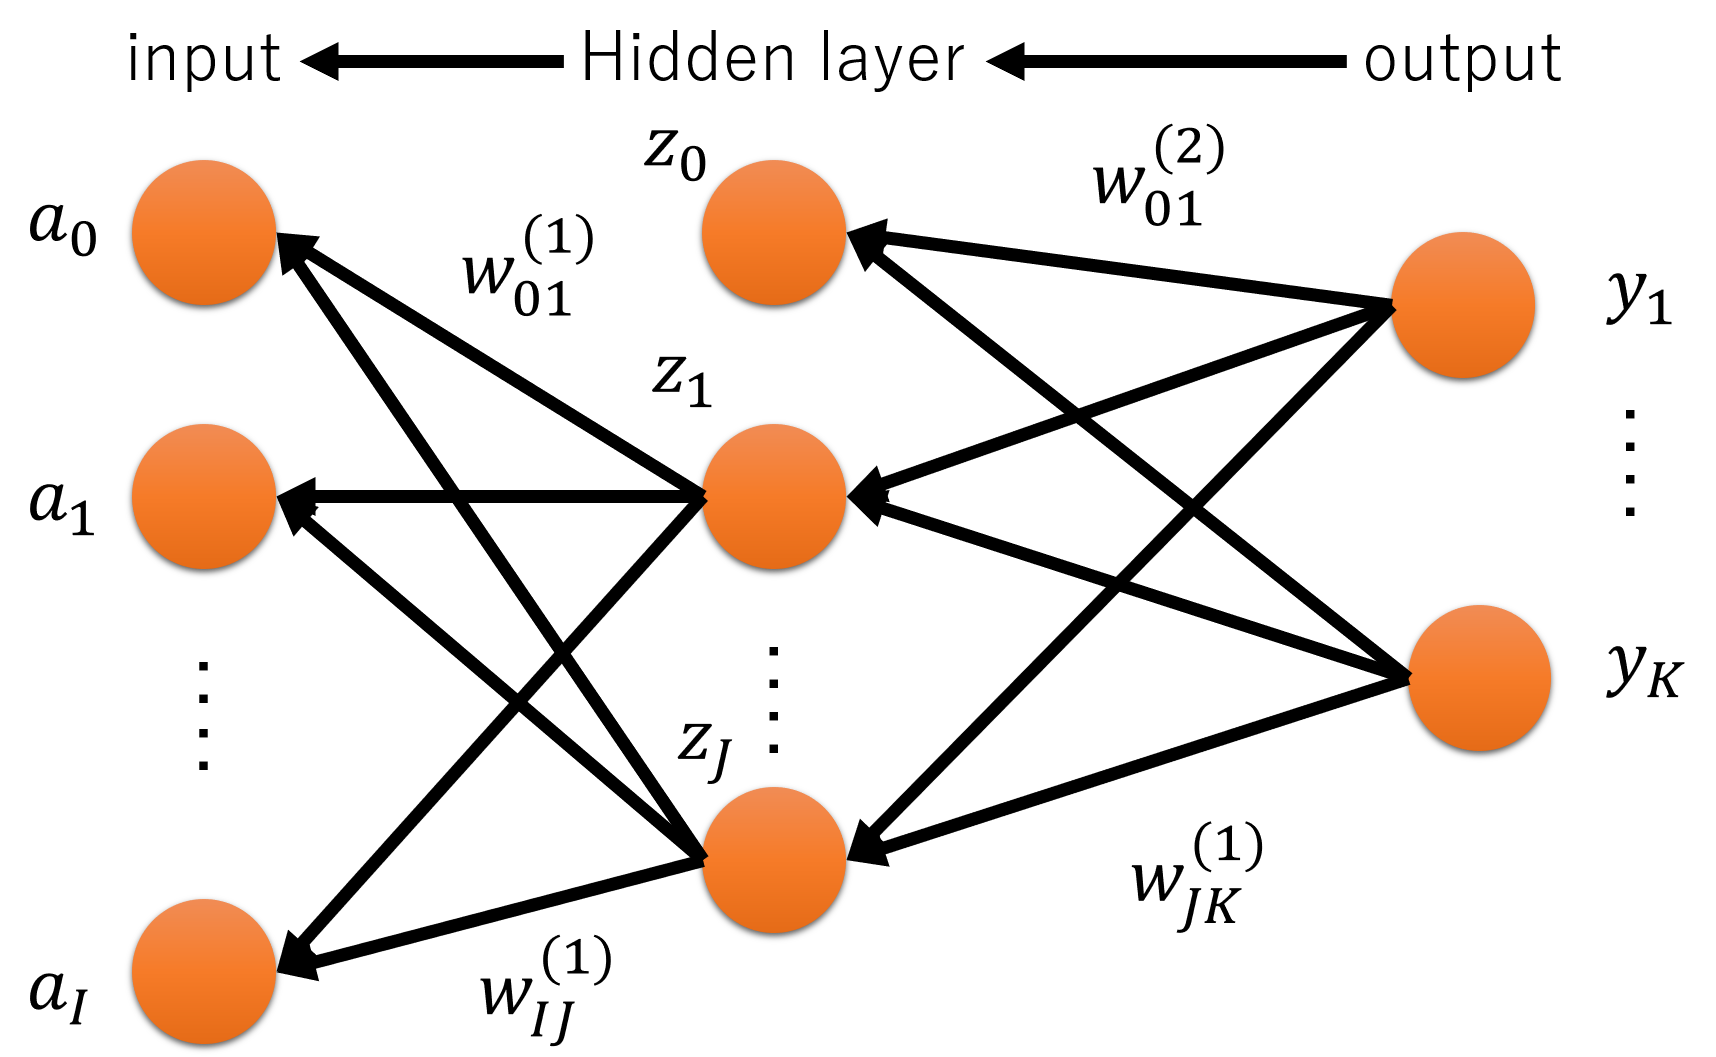
\includegraphics[scale=0.45]{figure5.png}
\caption{back-propagation}
\end{center}
\end{figure}
In learning, the goal is to bring the output ${\bm y}$ of the network
\begin{align}
{\bm y}=\left[\begin{array}{ccc}
	y_1 \\
	y_2 \\
	\vdots \\
	y_K
	\end{array}\right]
\end{align}
closer to the teacher vector (target vector) ${\bm t}$. That is, in learning, the weight $w$ is updated so as to minimize the error with the teacher vector. \par

Rumalhart et al.\cite{Rumelhart1986} proposed back-propagation as a method to update the parameter ${\bm w}$.
The back-propagation sometimes falls into the local optimum solution because it uses the steepest descent method. But practically it can get useful performance. Thus the back-propagation learning algorithm is the most popular learning algorithm for the multi layer perceptron. \par
The error function defined as the sum of training sample's error.
\begin{align}
E = \frac{1}{N}\sum_{n=1}^N{E_n}
\end{align} \par
We assumed that the error is given as
\begin{align}
E_n=\frac{1}{2}\sum_k{(y_{nk}-t_{nk})}^2
\end{align}
where $t_{nk}$ is the teacher signal of $k$-th output unit for $n$-th sample. \par
The gradient of $E_n$ using $w_{jk}$ is shown in Equation (\ref{gradient E}).
\begin{align} \label{gradient E}
\frac{\partial E_n}{\partial w_{jk}}&=\frac{\partial E_n}{\partial y_k} \frac{\partial y_k}{\partial w_{jk}} \\ \label{error}
\delta_k &\equiv \frac{\partial E_n}{\partial y_k}
\end{align}

Here, $\delta_k$ is called the error and is defined as shown in Equation (\ref{error}).
\begin{align}
\delta_k=\frac{\partial E_n}{\partial y_k}=\frac{\partial \frac{1}{2}\sum_k{(y_{nk}-t_{nk})}^2}{\partial y_{nk}}=y_{nk}-t_{nk}
\end{align}
From the Equations (\ref{gradient E}) and (\ref{error}), the following equation is obtained.
\begin{align} \label{gradient f1}
\frac{\partial E_n}{\partial w^{(2)}_{jk}}
&=\frac{\partial E_n}{\partial y_k}\frac{\partial y_k}{\partial w^{(2)}_{jk}}
=\delta_k \frac{\partial \sum_{j=1}^J{z_j w^{(2)}_{jk}}}{\partial w^{(2)}_{jk}} \\ \notag
\frac{\partial E_n}{\partial w^{(1)}_{ij}}
&=\frac{\partial E_n}{\partial z_j} \frac{\partial z_j}{\partial w^{(1)}_{ij}}
=\frac{\partial E_n}{\partial w^{(2)}_{jk}} \frac{\partial w^{(2)}_{jk}}{\partial z_j} \frac{\partial z_j}{\partial w^{(1)}_{ij}} \\ \notag
&=\frac{\partial E_n}{\partial y_k}\frac{\partial y_k}{\partial w^{(2)}_{jk}} \frac{\partial w^{(2)}_{jk}}{\partial z_j} \frac{\partial z_j}{\partial w^{(1)}_{ij}}
=\delta_k\frac{\partial y_k}{\partial w^{(1)}_{ij}} \\ \label{gradient f2}
&=\delta_k \frac{\partial h(\sum_{j=1}^J{z_j w^{(2)}_{jk}})}{\partial w^{(1)}_{ij}}
\end{align}
Therefore, the input data is transferred from the first layer to the last layer, and the errors that are gathered propagate from the final layer to the first layer. This is called back-propagation.
The $\frac{\partial E_n}{\partial w^{(l)}_{ij}}$ is used to update parameters with the stochastic gradient descent method(SGD). The general form of updating the weight is given as
\begin{align} \label{eq:sgd}
w^{(l)}_{ij} \leftarrow w^{(l)}_{ij}-\mu \frac{\partial E_n}{\partial w^{(l)}_{ij}}
\end{align}
Here, $\mu$ is called learning rate. Usually these parameters are updated by using the mini-batch approach in which the subsets of the training samples are used to calculate the partial derivatives. Also, from the time the whole training sample is obtained until the parameter is updated, it counts as one epoch.

The speed of optimization has been improved by adding momentum.
\begin{align} \label{eq:momentum}
w^{(l)}_{ij} \leftarrow w^{(l)}_{ij}-\mu \frac{\partial E_n}{\partial w^{(l)}_{ij}} + \eta \Delta w^{(l)}_{ij}
\end{align}
$\eta$ is the parameter of the momentum term, and $\Delta w^{(l)}_{ij}$ is the update amount of the weight of the previous iterator.
In our experiments, this was called SGD with momentum and used as an optimizer.

\subsection{Neural network for classification}

Let network output result and teacher vector be ${\bm y}$ and ${\bm t}$, respectively.

\begin{align}
{\bm y}=\left[\begin{array}{ccc}
	y_1 \\
    y_2 \\
    \vdots \\
    y_K
    \end{array}\right]\hspace{0.2cm}
{\bm t}=\left[\begin{array}{ccc}
	t_1 \\
	t_2 \\
	\vdots \\
	t_K
	\end{array}\right]
\end{align}
Here, ${\bm t}$ is one hot vector where $t_k (k=1,2,3,\cdots,K)$ corresponds to class $k$ in which a single output that relates to certain class is 1 and the others are 0. \par

Softmax cross entropy error is as



\begin{align} \label{crossentropy}
E=-\sum_{n=1}^N \sum_{k=1}^K{t_{nk}log(S_k({\bm y}_n))}
\end{align}
Here, $S_k({\bm y}_n)$ is as follows,
\begin{align} \label{softmax}
S_k({\bm y}_n) = \frac{exp(y_{nk})}{\sum_{k^\prime=1}^K{exp(y_{k^\prime})}}
\end{align}
Equation (\ref{softmax}) is called a softmax function, and it is used as an activation function of the output unit in classification. \par
As in Section 2.1, Based on the error $\delta_k$ from Equation (\ref{crossentropy}).
\begin{align}
\frac{\partial E_n}{\partial y_{nk}} &=-\sum_{i=1}^K{\frac{\partial E_n}{\partial S_i} \frac{\partial S_i}{\partial y_{nk}}}=-(\frac{\partial E_n}{\partial S_k}\frac{\partial S_k}{\partial y_{nk}}+\sum_{i \neq k}{\frac{\partial E_n}{\partial S_i} \frac{\partial S_i}{\partial y_{nk}}}) \notag \\
&=-\frac{\partial E_n}{\partial S_k} \{S_k(1-S_k)\}-\sum_{i \neq k}{\frac{\partial E_n}{\partial S_i}(-S_i S_k)} \notag \\
&=-\frac{t_{nk}}{S_k}\{S_k(1-S_k)\}+\sum_{i \neq k}{\frac{t_{ni}}{S_i}(S_i S_k)} \notag \\
&=-t_{nk}(1-S_k)+\sum_{i \neq k}{t_{ni} S_k}=-t_{nk}+\sum_i{t_{nk} S_i} \notag \\
&= S_k - t_{nk}=\delta_k
\end{align}
An error shown in Equation (\ref{error}) is derived by derivative of softmax cross entropy with respect to input $y_k$.
Therefore, errors are propagated to the input by back-propagation as in Equations (\ref{gradient f1}) and (\ref{gradient f2}), and the weight $w^{(l)}_{ij}$ is updated. Also, $t_k$ is 1 only when the input belongs to class $k$, and 0 otherwise. Therefore $S_k$ can be regarded as the probability that input belongs to class $k$. 
The network judges that certain input belongs to class $k$ when the probability $S_k$ is the highest.
Classification by network is realized in this manner.



%From equation(2), $S(x_i)$ can be seen as the probability that $x_i$ belongs to class $i$. That is, the probability that the input belongs to the class $i$ is higher as the value of $x_i$ is larger. \par
%Let $x$ and $y$ denote model outputs and teacher labels when samples belonging to class 1 are input.

%Here, the teacher vector is a vector in which only elements corresponding to the respective classes are 1 and the others are 0. 









Furthermore, neural network sometimes depend on training samples. This state is called over learning. In order to prevent this, we often add a regularization term to error function. The simplest form of regularization terms is the sum of squares of the weights ${\bf w}$.(Equation (\ref{weightdecay}))
\begin{align} \label{weightdecay}
E_W=\frac{1}{2}{\bm w}^T{\bm w}
\end{align}
If we use this as a regularization term, the error function is rewritten as follows.
\begin{align}
E^\prime=E + \frac{1}{2}\gamma{\bm w}^T{\bm w}
\end{align}
Here, $\gamma$ is a regularization coefficient that controls the effect of regularization term, and it is determined artificially. The implementation of this term is called weight decay and is often used when learning the model.

\clearpage
\subsection{Deep Convolutional Neural Network}
\begin{figure}[ht]
\begin{center}
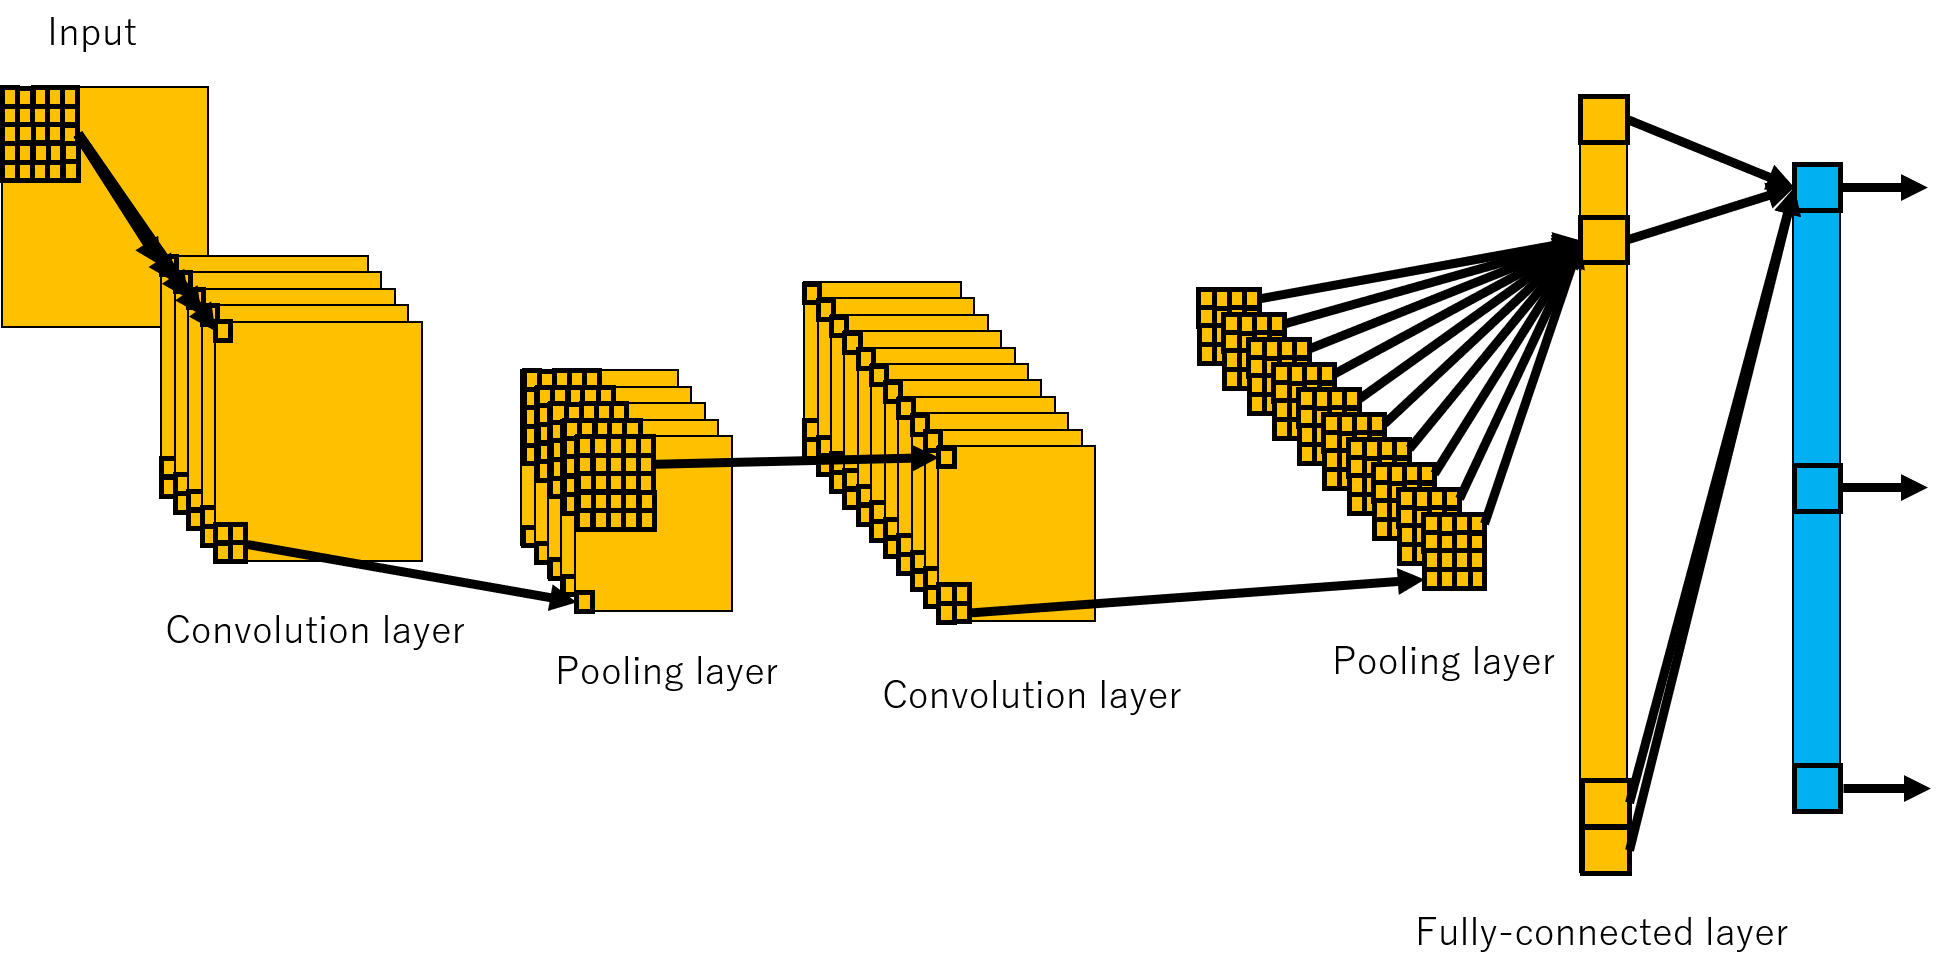
\includegraphics[scale=0.4]{figure8.png}
\caption{This is the figure of deep convolutional neural network. Convolution layer and pooling layer are connected and followed by fully connected layer and classification layer.}
\end{center}
\end{figure}

%As mentioned above, since Krizhevsky et al. found that the Deep Convolutional Neural Network has the top performance in image classification in 2012, this model has become widely used in image classification.\par




The deep convolutional neural network (CNN) is effective for image classification tasks.
The network architecture is originally designed by imitating the visual information processing in our brain. 
The deep CNN consists of multiple convolution layers which are corresponding to the neuron with receptive field in the primal visual cortex and fully connected layers for classifier.\par

The convolution layer is the core building block of a deep CNN. Each neuron of the convolution layer can be regarded as a learnable filter. The neurons are tiled in a way that the neurons receptive fields cover the entire input image as shown in Figure 3. The weights of the neurons in the array are shared. Through the weight sharing, the computation within the neurons becomes a filtering process of the input image as
\begin{align}
f_{p,q}^{(l)}=h(\sum^{convy-1}_{s=0}\sum^{convx-1}_{t=0}w^{(l)}_{s,t}f^{(l-1)}_{p+s, q+t}+b^{(l)})
\end{align}
where $w^{(l)}_{s,t}$ is the weight of the neuron indexed as $(s,t)$ in the $l$-th convolution layer and $b^{(l)}$ is the bias of the $l$-th convolution layer. Furthermore, the size of the convolution filter is $convx \times convy$. $h$ is the activation function. For simplicity, it is assumed that the activation function is Relu, and only the case of $f^{(l)}_{p,q} \geq 0$ is considered here. so,
\begin{align}
f_{p,q}^{(l)}=h(\sum^{convy-1}_{s=0}\sum^{convx-1}_{t=0}w^{(l)}_{s,t}f^{(l-1)}_{p+s, q+t}+b^{(l)})=\sum^{convy-1}_{s=0}\sum^{convx-1}_{t=0}w^{(l)}_{s,t}f^{(l-1)}_{p+s, q+t}+b^{(l)}
\end{align}

\begin{figure}[ht]
\begin{center}
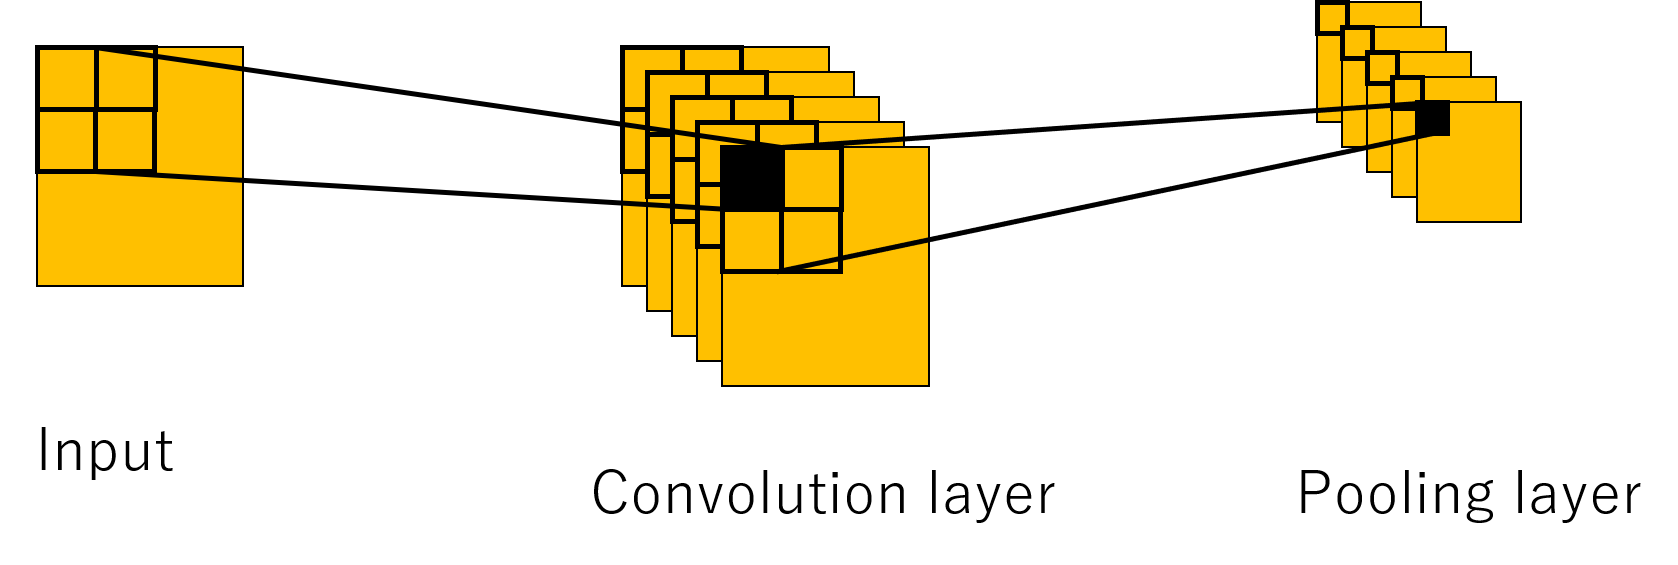
\includegraphics[scale=0.4]{figure12.png}
\caption{The pair of the convolution and the pooling layers.}
\end{center}
\end{figure}
If there are several channels in the input layer, the sum of the filtered outputs are used as the activity of the neuron. Thus the array of the neurons with the same weights is produced. This is called as feature map. \par
Thus the network can learn filters that activate when they encounter some specific type of feature at some spatial position in the input. Since the weight sharing reduces the number of parameters drastically, the computation for learning is reduced and also the generalization of the trained network is improved when compared to the multi layer perceptron. \par
Shows the back-propagation of the convolution layer. As shown in Equation (\ref{converror}), an error $\delta_{p,q}^{(l)}$ is defined.
\begin{align} \label{converror}
\delta^{(l)}_{p,q} \equiv \frac{\partial E_n}{\partial f_{p,q}^{(l)}}
\end{align}
Equation (\ref{converror}) is transformed as follows.
\begin{align} \label{calc converror}
\delta^{(l)}_{p,q}&=\frac{\partial E_n}{\partial f_{p,q}^{(l)}}=\sum_{s=0}^{convy-1}\sum_{t=0}^{convx-1}{\frac{\partial E_n}{\partial f^{(l+1)}_{p-s,q-t}}\frac{\partial f^{(l+1)}_{p-s,q-t}}{\partial f^{(l)}_{p,q}}} \notag \\
&=\sum_{s=0}^{convy-1}\sum_{t=0}^{convx-1}{\delta^{(l+1)}_{p-s,q-t}\frac{\partial f^{(l+1)}_{p-s,q-t}}{\partial f^{(l)}_{p,q}}}
\end{align}
Here, $\frac{\partial f^{(l+1)}_{p-s,q-t}}{\partial f^{(l)}_{p,q}}$ is calculated as follows.
\begin{align}
\frac{\partial f^{(l+1)}_{p-s,q-t}}{\partial f^{(l)}_{p,q}}&=\frac{\partial}{\partial f^{(l)}_{p,q}}\sum^{convy-1}_{s^{\prime}=0}\sum^{convx-1}_{t^{\prime}=0}{w^{(l+1)}_{s^\prime,t^\prime}f^{(l)}_{p-s+s^\prime, q-t+t^\prime}+b^{(l+1)}} \notag \\
&=w^{(l+1)}_{s,t}
\end{align}
Substituting into Equation (\ref{calc converror}) results in,
\begin{align}
\delta^{(l)}_{p,q} = \sum_{s=0}^{convy-1}\sum_{t=0}^{convx-1}{\delta^{(l+1)}_{p-s,q-t}w^{(l+1)}_{s,t}}
\end{align} \par
From the Equation (\ref{converror}), the following equation is obtained. Where $m$ and $n$ are the size of the input.

\begin{align} \label{gradient conv}
\frac{\partial E_n}{\partial w^{(l)}_{s,t}}&=\sum_{p=0}^{m-convy}\sum_{q=0}^{n-convx}{\delta^{(l)}_{p,q}\frac{\partial f_{p,q}^{(l)}}{\partial w^{(l)}_{s,t}}} \notag \\
&=\sum_{p=0}^{m-convy}\sum_{q=0}^{n-convx}{\delta^{(l)}_{p,q}f^{(l-1)}_{p+s, q+t}} \\
\frac{\partial E_n}{\partial b^{(l)}} &= \sum_{p=0}^{m-convy}\sum_{q=0}^{n-convx}{\delta^{(l)}_{p,q}\frac{\partial f_{p,q}^{(l)}}{\partial b^{(l)}}} \notag \\
&=\sum_{p=0}^{m-convy}\sum_{q=0}^{n-convx}{\delta^{(l)}_{p,q}}
\end{align}
Therefore, it can be seen that the error propagates to the previous layer.



Usually pooling layers are inserted after the convolution layers.
The pooling layer performs down sampling, thereby reducing computational costs and enhancing against micro position changes. There are two types of pooling methods: average pooling and max pooling.
The average pooling samples the average value within a certain region of the feature map and compresses the feature map. Max pooling samples the maximum value within a certain region of the feature map and compresses the feature map. While average pooling was historically used, max pooling, which has been proven to be more effective, is now in use.





There are fully-connected layer like multi layer perceptron behind the convolution layer. It specifies how the network training penalizes the deviation between the predicted and true labels.
The feature map obtained in the last convolution layer $f^{(r)}_{p,q}$ is input to the fully-connected layer in the form of $a_{p*convx+q}$ vector.  \par
That is,
\begin{align} \label{full input}
f^{(r)}_{p,q}=a_{p*convx+q}
\end{align}
Therefore, the error $\delta^{(r)}_{p,q}$ of the last convolution layer is expressed as follows using weights $w_{ij}^{(1)}$, $w_{jk}^{(1)}$ of the fully-connected layer.
\begin{align} \label{last converror}
\delta^{(r)}_{p,q}&=\frac{\partial E_n}{\partial f_{p,q}^{(r)}}=\frac{\partial E_n}{\partial a_{p*convx+q}} \notag \\
&=\sum_{j=1}^{J}{\frac{\partial E_n}{\partial z_j}\frac{\partial z_j}{\partial a_{p*convx+q}}} \notag \\
&=\sum_{j=1}^{J}{\frac{\partial E_n}{\partial y_k}\frac{\partial y_k}{\partial z_j}\frac{\partial z_j}{\partial a_{p*convx+q}}} \notag \\
&=\sum_{j=1}^{J}{\delta_kw^{(2)}_{jk}w^{(1)}_{p*convx+qj}}
\end{align}
So, it is understood that the error $\delta_k$ obtained from the output of the fully-connected layer propagates to the convolution layer.
The error of the last fully-connected layer propagates to the convolution layer of the input by back-propagation.

\subsection{Metric Learning}
Metric learning is a method of learning embedding for metric (Euclidean distance, cosine similarity, etc.).
Metric learning is applied to a wide range of tasks such as image search, biometric authentication, and abnormality detection.

\begin{figure}[ht]
\begin{center}
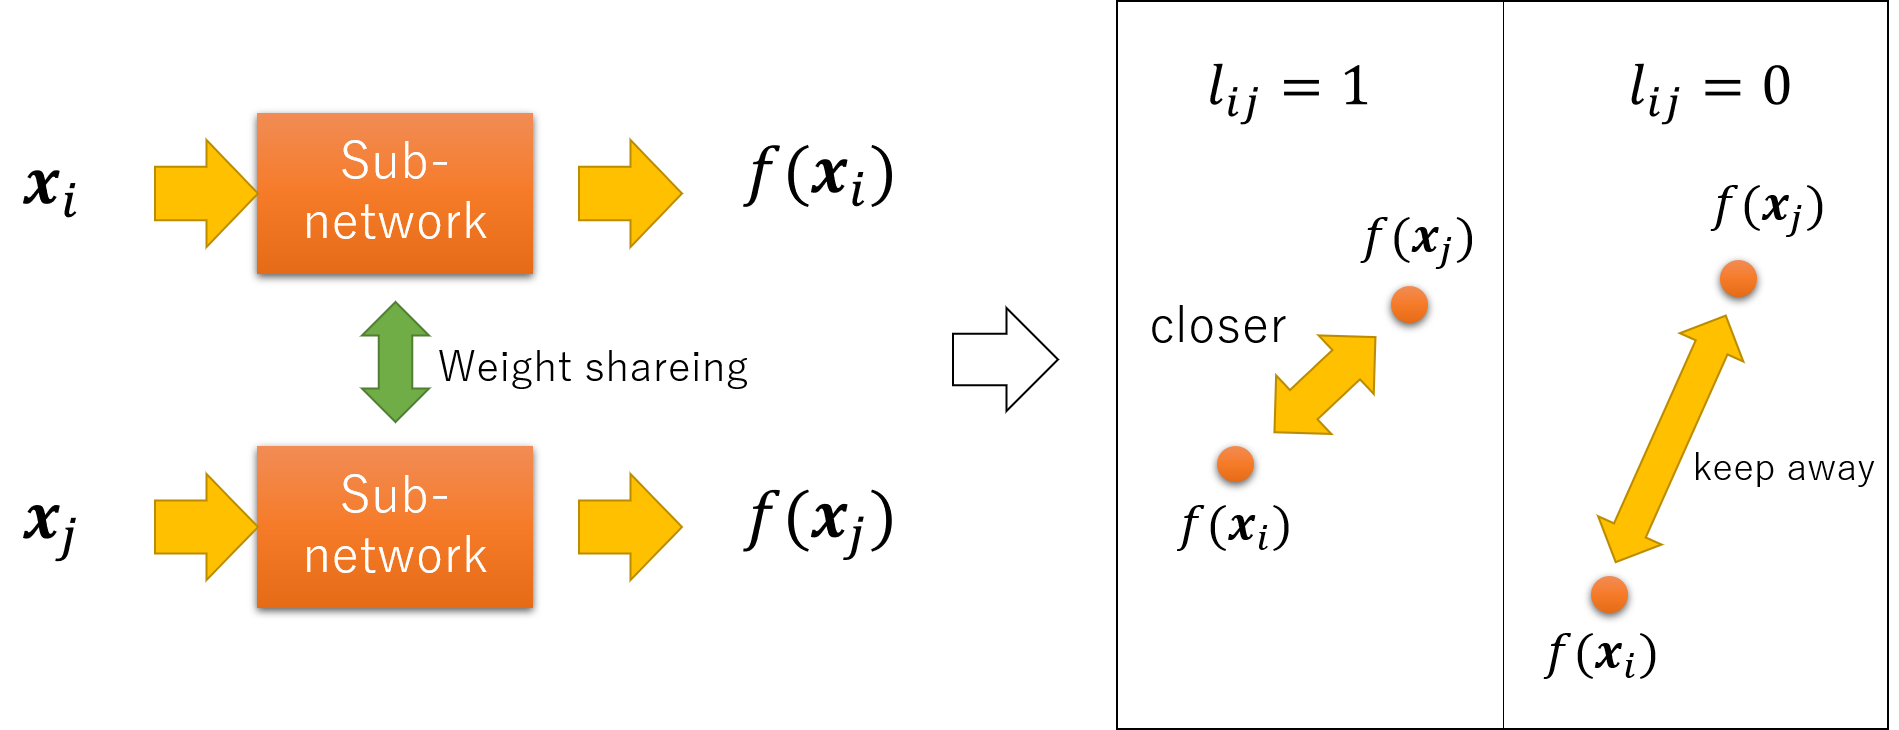
\includegraphics[width=80mm]{figure_siamese.png}
\caption{The structure of Siamese Network. The distance metric is learned depending on the label $l_{ij}$ given to each sample pair $\bm{x}_i$ and $\bm{x}_j$.}
\label{fig:siamese}
\end{center}
\end{figure}

A typical model for deep learning embedding is the Siamese Neural Network \cite{Bromely1994,Chopra2005,Hadsell2006}.
The Siamese Network consists of two identical networks joined at their outputs.
The two networks extract feature vectors from two different samples.
Usually, the weights of the two networks are shared.
The objective function of the optimization for training the parameters of the networks is defined by using these extracted feature vectors as
\begin{align} \label{eq:contrastive}
E=\frac{1}{2|\chi^2|}\sum_{(i,j) \in \chi^2} l_{ij}(D_{ij})^2 + (1-l_{ij})max(m-D_{ij}, ~0)^2 \; ,
\end{align}
where $D_{ij}$ represents the distance between the pair of the outputs $f(\bm{x}_i)$ and $f(\bm{x}_j)$ of each network for the sample pair $\bm{x}_i$ and $\bm{x}_j$.
The distance $D_{ij}$ is defined by
\begin{align} 
D_{ij}&=||f({\bm x}_{i})-f({\bm x}_{j})||_2 \; ,
\label{eq:dis}
\end{align}
where $m$ is a parameter indicating the distance between clusters and 
$\chi^2$ is an index set of sample pairs randomly generated from the samples in the mini-batch.
A label $l$ is assigned for each sample pair such that 
label is $l_{ij}=1$ when the pair $i$ and $j$ is similar and label is $l_{ij}=0$ when the pair $i$ and $j$ is dissimilar.
The scheme of Siamese Network is shown in Fig. \ref{fig:siamese}.

After the training of Siamese Network, the distance between the outputs for dissimilar pair will be far while the distance between the outputs for similar pair become close.
The Siamese Network can only consider the metric between samples pairwise.
For this reason, the Siamese Network have to uniquely determine the concept of similarity.
For example, if there are two different male images, in the case of the concept of “gender”, they should be judged to be similar.
However, in the case of the concept of “individuals”, they should be judged not to be similar.
It is difficult to express these multiple concepts in the Siamese Network.

Wang et al. \cite{Wang2014}, Hoffer et al. \cite{Hoffer2015} proposed the Triplet Network (Figure \ref{fig:triplet}), an extension of the Siamese Network to triplet-wise.

\begin{figure}[ht]
\begin{center}
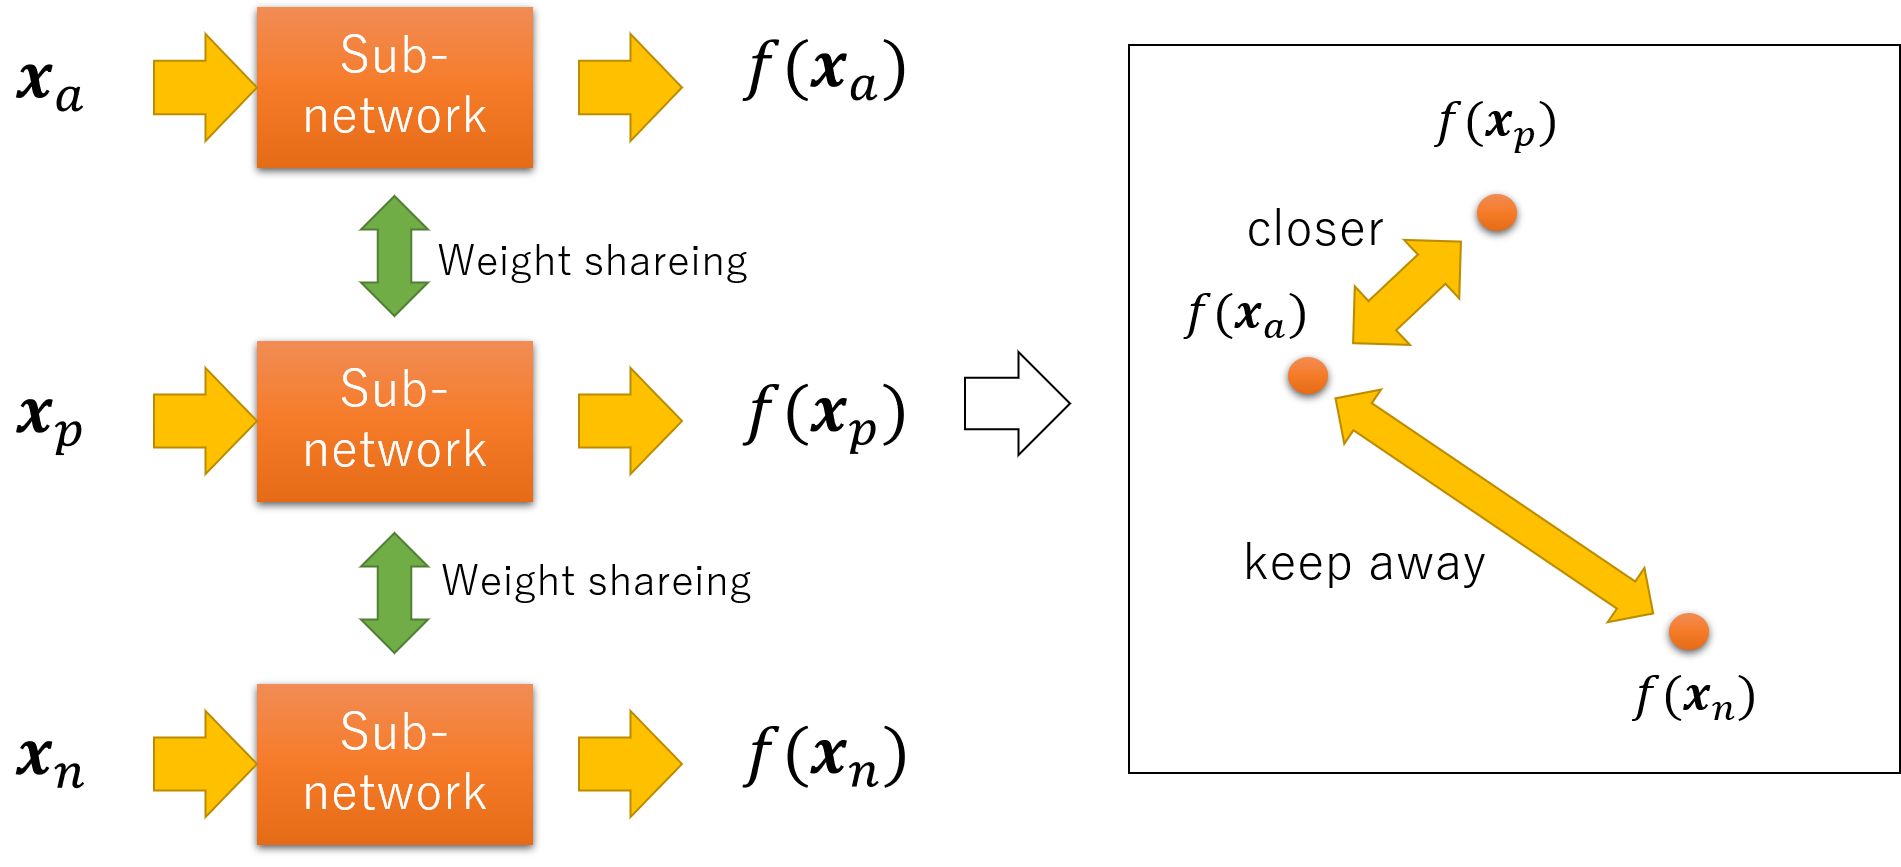
\includegraphics[width=80mm]{figure_triplet.png}
\caption{The structure of Triplet Network. The distance metric is learned by using three networks with the shared weights from triplet $\bm{x}_a$, $\bm{x}_p$ and $\bm{x}_n$ which are called "anchor", "positine", and "negative". Learning progresses as closer "anchor-positive", and keep away "anchor-negative".}
\label{fig:triplet}
\end{center}
\end{figure}

Triplet Network is designed to learn embedding from a triplet of samples called "anchor", "positive" and "negative".
The triplet network learns embedding such that the distance between "anchor" ${\bm x_a}$ and "positve" ${\bm x_p}$ is smaller than the distance between "anchor" ${\bm x_a}$ and "negative" ${\bm x_n}$.
Various losses have been proposed for the Triplet Network.
The triplet loss 
\begin{align} \label{eq:triplet}
    E=\sum_{(a,p,n) \in \Theta}max(0, m + ||f({\bm x_a})-f({\bm x_p})||_2^2 - ||f({\bm x_a}) - f({\bm x_n})||_2^2)
\end{align}
is generally used, 
where $f(\cdot)$ denotes the output of the model, and $m$ is a parameter indicating the distance between clusters.
$\Theta$ is an index set of "anchor", "positive", and "negative".
The triplet network learns so that the anchor-positive distance is relatively closer than the anchor-negative distance.
Therefore, multiple similar concepts can be considered without depending on one similar concept.
Triplet Network can overcome the drawbacks of Siamese Network.



\subsection{RankSVM}
The RankSVM is a ranking model minimizing margin-based pairwise loss \cite{Herbrich2000}.
RankSVM was trained to minimize the loss function defined by
\begin{align} \label{eq:RankSVM}
    \frac{1}{2}||{\bm w}||^2+\lambda \sum_{i \in P, j \in N}max(0, 1-{\bm w}^T({\bm x}_i - {\bm x}_j))^2
\end{align}
where $P$ is a set of positive training samples, and $N$ is a set of negative training samples. 
$\lambda$ is a parameter of $\lambda > 0$, ${\bm w}$ is a weight.
And $({\bm x}_i, {\bm x}_j)$ is a pair of training samples given a positive label and a negative label.
As can be seen from equation (\ref{eq:RankSVM}), among the pairs of the positive vector and the negative vector, the loss becomes large when the pair is incorrectly ranked.

O. Chapelle et al. \cite{Chapelle2010} proposed a fast optimization method for RankSVM based on the primal Newton method.
Also, O. Chapelle et al. showed that RankSVM can be used for binary classification and can improve area under the ROC curve (AUC) defined as 
%(Equation(\ref{eq:AUC})) as a evaluation criterion.
\begin{align} \label{eq:AUC}
    AUC=\frac{|\{(i,j)| t_i=1, t_j=0, \bm{y}_i > \bm{y}_j \}|}{|\{i|t_i=1\}| \times |\{j|t_j=0\}|}
\end{align}
where $t_i \in \{1,0\}$ is a label assigned to $i$-th training sample and $|S|$ denotes the number samples in the set $S$.
$\bm{y}_i$, $\bm{y}_j$ are outputs of RankSVM for samples ${\bm x}_i$, ${\bm x}_j$.
\begin{figure}[ht]
\begin{center}
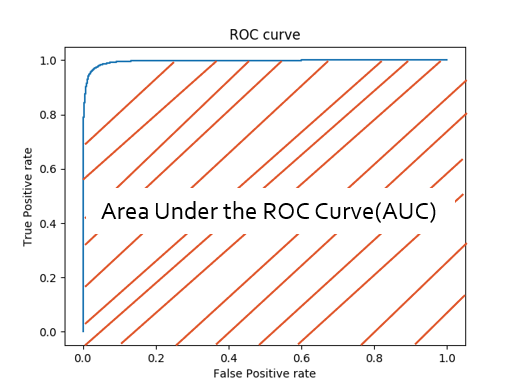
\includegraphics[width=70mm]{figure_ROC.png}
\caption{ROC curve}
\label{fig:triplet}
\end{center}
\end{figure}
The ROC curve is a plot in which the vertical axis represents the True Positive Rate of the model and the horizontal axis represents the False Positive Rate.
True Positive Rate is a rate at which a sample of class “0” was identified as class “0” in the binary classification of class “0” and class “1”.
False Positive Rate is the rate at which samples of class "1" were incorrectly identified as class "0".
So, the larger the area under the ROC curve (AUC) is, the more suitable the model is for discriminating between a sample of class "0" and a sample of class "1".

The denominator is the product of the number of positive samples and the number of negative samples and the numerator is the number of pairs that positive and negative samples could be classified correctly.
In order to optimize the loss defined by the equation (\ref{eq:RankSVM}), the ranking of ${\bm x_i}$ and ${\bm x_j}$ must be correct.
That means that the AUC score should be high. 
This has been introduced as a special case of RankSVM.
\clearpage
\subsection{Knowledge Distillation}
\begin{figure}[ht]
\begin{center}
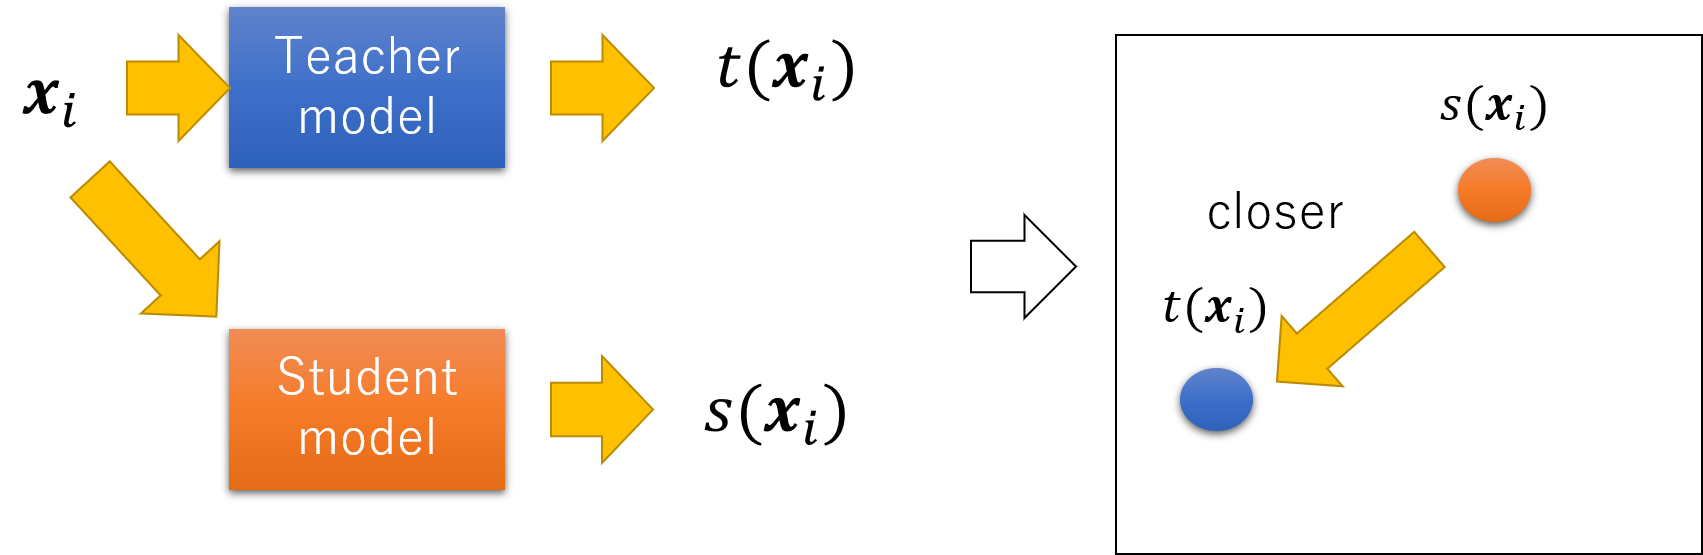
\includegraphics[width=80mm]{figure_KD.png}
\caption{The structure of conventional knowledge distillation. The student model tries to mimic the teacher model.}
\label{fig:KD}
\end{center}
\end{figure}
Knowledge distillation is a technique for transferring knowledge of deep or ensemble model with many parameters (teacher model) to smaller shallow model (student model).
Various approaches have been proposed for transferring knowledge.

Ba et al. \cite{Ba2014} considered the difference between the input vectors of the softmax actication function (logits) of the teacher model and the student model as loss (Equation(\ref{eq:Ba})), and proposed to train the student model so that the feature vectors of the student model got close to the teacher model (BKD).
The loss to measure the similarity between the teacher model and the student model is defined by the mean squared errors between the feature vector $t(\cdot)$ of the teacher model and the feature vector $s(\cdot)$ of the student model as 
\begin{align} \label{eq:Ba}
E_{BKD}= \frac{1}{2}\sum_{i \in \chi} ||t(\bm{x}_i) - s(\bm{x}_i)||^2_2,
\end{align}
where $\chi$ is the set of training samples.
%This loss is minimized to train the parameters of the student model.
As a result, the authors found that the performance of the student model was higher than the network trained by the student model alone.
They claimed that the uncertainty of the feature vectors of the teacher model is useful for learning the student model.

Hinton et al. \cite{Hinton2015} proposed training the student model so that the softmax outputs of the teacher model and the softmax outputs (probability) of the student model are close (HKD).
They used the KL-divergence of the softmax outputs of both models as the loss for training the student model.
The loss based on the KL-divergence is defined as
\begin{align} \label{eq:Hinton}
    E_{HKD} = \sum_{i \in \chi} KL(\mbox{softmax}(\frac{t(\bm{x}_i)}{T}), \mbox{softmax}(\frac{s(\bm{x}_i)}{T})),
\end{align}
where $\mbox{softmax}(\cdot)$ is the softmax function,
$KL(\cdot)$ is KL-divergence between the softmax outputs of the teacher model $\{p_i\}$ and the softmax outputs $\{q_i\}$ of the student model defined by
\begin{align} \label{eq:KL-divergence}
KL(\bm{p}, \bm{q}) = \sum_{i} p_i log(\frac{p_i}{q_i}) \; ,
\end{align}
and $T$ is a temperature parameter.
They argued that negative values in logits could have a positive effect in some cases or negative effect in some cases, on learning.


In recent years, various approaches have been proposed for knowledge distillation.
Park et al. \cite{Park2019} expressed the relationship between the outputs of the teacher model as the Euclidean distance between the two outputs, and transferred it to the student model (RKD-D).
They expressed the similarity between the pair of the outputs $t(\bm{x}_i$ and $t(\bm{x}_j)$ as
\begin{align} \label{eq:psiD}
    \psi_D(t(\bm{x}_i), t(\bm{x}_j)) = \frac{||t(\bm{x}_i) - t(\bm{x}_j)||_2}{\sum_{(\bm{x}_i, \bm{x}_j) \in \chi^2} ||t(\bm{x}_i) - t(\bm{x}_j)||_2},
\end{align}
where $\chi^2$ is a set of sample pairs randomly generated from the samples in the mini-batch.
They optimized the student model by Huber loss so that the similarity between the outputs of the student model and the similarity of the outputs of the teacher model got closer.
%(Equation(\ref{eq:RKD-Dloss})).
The loss function of RKD-D is defined by using the similarity $\psi_D$ as
\begin{align} \label{eq:RKD-Dloss}
    E_{RKD-D} = \sum_{(\bm{x}_i, \bm{x}_j) \in \chi^2} l(\psi_D(t(\bm{x}_i), t(\bm{x}_j)), \psi_D(s(\bm{x}_i), s(\bm{x}_j)),
\end{align}
where
\begin{eqnarray} \label{eq:Huber}
l(p,q)=\left\{
\begin{array}{ll}
\frac{1}{2}(p-q)^2 & (|p-q| \leq 1) \\
|p-q|-\frac{1}{2} & (otherwise)
\end{array}
\right. \; 
\end{eqnarray} 
is Huber loss.

They also used the cosine of the angle formed by the three outputs as the similarity of the model outputs (RKD-A).
The cosine of the three outputs $t(\bm{x}_i)$, $t(\bm{x}_j)$, and  $t(\bm{x}_k)$ is defined by
\begin{align} \label{eq:psiA}
    &\psi_A^{(t_{ijk})} = \cos \angle t(\bm{x}_i) t(\bm{x}_j) t(\bm{x}_k),
\end{align}
where
\begin{align} \label{eq:psiA-cos}
 \cos \angle t(\bm{x}_i) t(\bm{x}_j) t(\bm{x}_k) &= \langle \bm{e}^{(t_{ij})}, \bm{e}^{(t_{kj})} \rangle
\end{align}
\begin{align}
    \bm{e}^{(t_{ij})} &= \frac{t(\bm{x}_i) - t(\bm{x}_j)}{||t(\bm{x}_i) - t(\bm{x}_j)||_2}, \notag \\ \bm{e}^{(t_{kj})} &= \frac{t(\bm{x}_k) - t(\bm{x}_j)}{||t(\bm{x}_k) - t(\bm{x}_j)||_2} \; .
\end{align}
Loss of RKD-A is also defined by using Huber loss \cite{Huber1992} as
\begin{align} \label{eq:RKD-Aloss}
E_{RKD-A} = \sum_{(\bm{x}_i, \bm{x}_j, \bm{x}_k) \in \chi^3}l(\psi_A^{(t_{ijk})}, \psi_A^{(s_{ijk})}) \: ,
\end{align}
where $\chi^3$ is a set of triplet samples randomly generated from the samples in the mini-batch.

They also argued that using both angles and Euclidean distance for knowledge transfer would further improve the performance of the student model (RKD-DA).
The loss for this case is defined as
\begin{align} \label{eq:RKD-DAloss}
E_{RKD-DA} = \lambda_{RKD-D} E_{RKD-D} + \lambda_{RKD-A} E_{RKD-A} \; ,
\end{align}
where $\lambda_{RKD-D}$ and $\lambda_{RKD-A}$ are the hyper-parameters.

\begin{figure}[ht]
\begin{center}
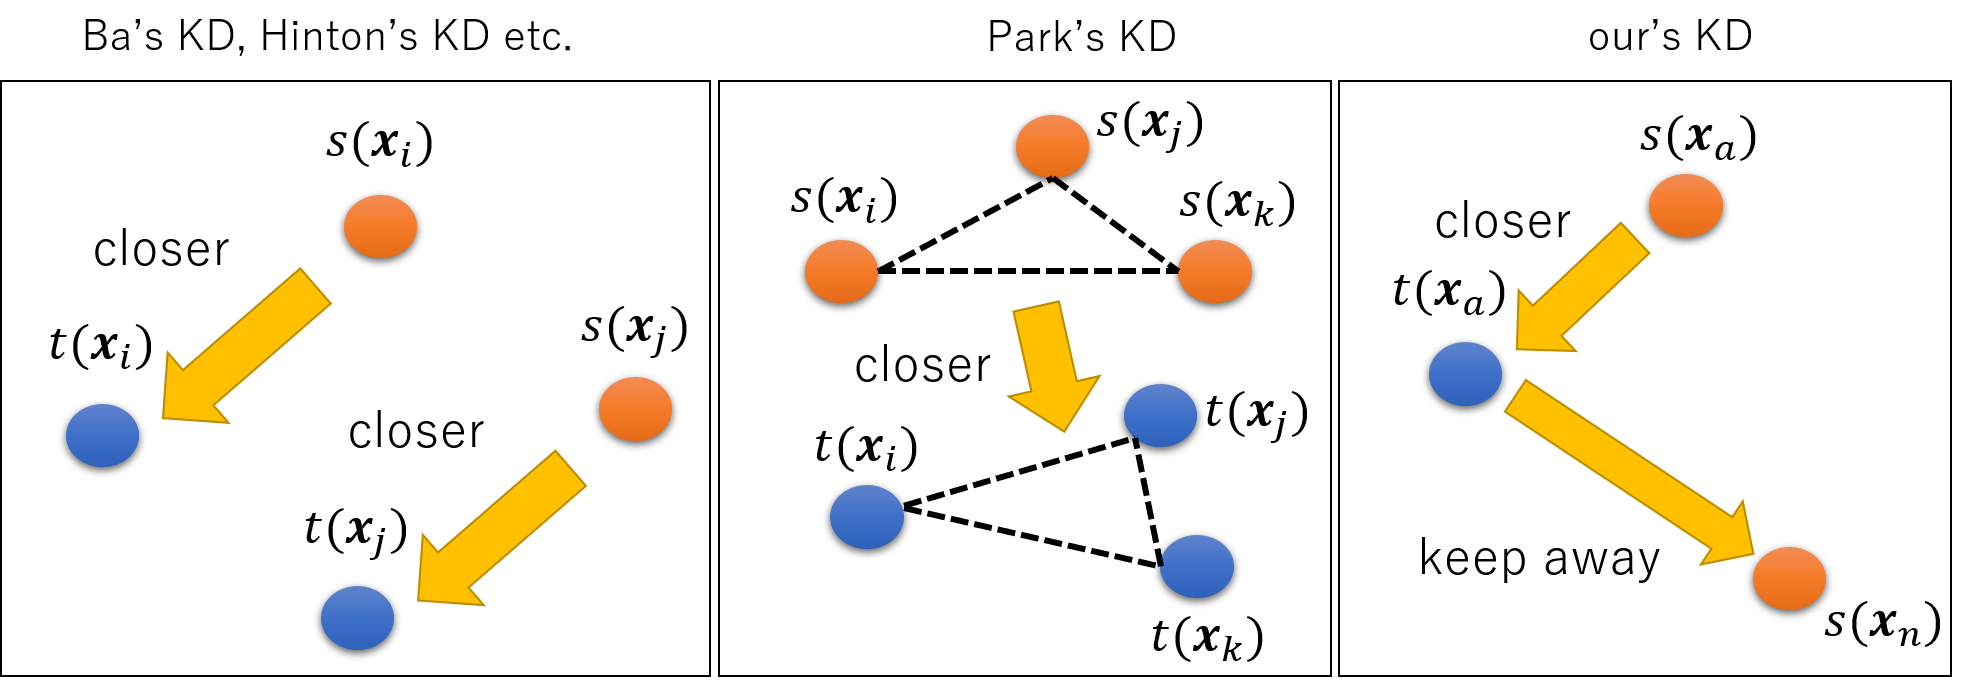
\includegraphics[width=80mm]{figure_structure.png}
\caption{The summary of knowledge distillation methods in terms of the loss function.}
\label{fig:loss}
\end{center}
\end{figure}

The pair-wise or triplet-wise similarity between the output of the teacher model to the output of the student model is considered in RKD-D, RKD-A, or RKD-DA while the point-wise transfer was performed in the knowledge distillation methods such as Ba's KD \cite{Ba2014} or Hinton's KD \cite{Hinton2015}.
Thus the knowledge distillation methods such as RKD-D, RKD-A, or RKD-DA succeeded in achieving top performance.


The loss using the output distribution of the teacher model (soft target) can be used alone or combined with the loss using the label of the original training data (hard target).
The combined loss can be defined as
\begin{align} \label{eq:distillation loss}
E_{KD} = E_{hard} + \lambda_{soft} E_{soft},
\end{align}
where $E_{hard}$ is hard target loss and $E_{soft}$ is soft target loss.
In this case, a hyper-parameter $\lambda$ is introduced to keep the balance between the hard target and the soft target.
It is also possible to combine multiple soft target losses.
For example, in Park's KD, they are $\lambda_{RKD-D}$ and $\lambda_{RKD-A}$.
%In this case, each loss is weighted.



\section{Our Works}
We tried to apply metric learning to AUC optimization in image classification and transfer of knowledge from teacher model to student model in knowledge distillation.
Each section discusses each of these in detail.
\subsection{Metric Learning for optimization of AUC}
O. Chapelle et al. \cite{Chapelle2010} show that RankSVM can be used to construct a binary classifier for optimizing the AUC.
%RankSVM can learn ranking.
Binary classification is realized by using RankSVM and by maximizing the margin of positive sample and negative sample. 
%Also, the authors show that RankSVM can be used to construct a binary classifier for optimizing the AUC.
%In other words, RankSVM assumes that a positive sample and a negative sample are input as a pair, and it learns their ranking.
Since the Siamese Network for rank learning uses the same loss function with RankSVM,
the Siamese Network also can be used to construct a binary classifier for optimizing the AUC.
%learn to output the similar feature vectors to the samples in the same class and to output different feature vectors for the samples of different classes.
%And, in addition to ranking positive samples and negative samples, the Siamese Network also learns the relationship between samples of the same class.
%Therefore, in classification, we think that Siamese Network also can optimize AUC like RankSVM. 
In this section, we propose to use the Siamese Network for rank learning for constructing a binary classifier.
Then the proposed method is extended to multi-class classification problem.
\clearpage

\subsubsection{Binary Classification}
\begin{figure}[ht]
\begin{center}
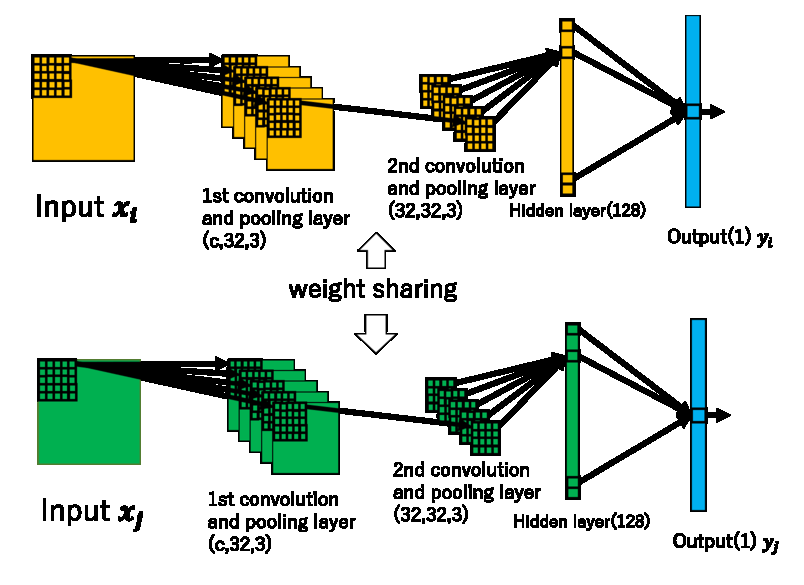
\includegraphics[width=100mm]{figure2.eps}
\caption{Siamese Network for binary classification}
\label{fig:siamese-bi}
\end{center}
\end{figure}

In order to perform binary classification, consider the Siamese Network which classify the positive class and the negative class as shown in Figure \ref{fig:siamese-bi}.
The output of each network $y$ is assumed to be scalar, namely the dimension of the output is $1$.
Similar with the standard Siamese Network, the weights of the two networks are shared.
ReLU is used as an activation function for each convolution layer and hidden layer.


The objective function of the Siamese Network for binary classification is defined as
\begin{align}
E&=\frac{1}{2|\chi^2|}\sum_{(i,j) \in \chi^2} l_{ij}(D_{ij})^2 + (1-l_{ij})max(m-D_{ij}, ~0)^2 \\
D_{ij}&=||y_{i}- y_{j}||^2_2
\label{eq:siamese-dis}
\end{align}
where $\chi^2$ is an index set of sample pairs randomly generated from the mini-batch, $m$ is a parameter indicating the distance between clusters and 
$D_{ij}$ is the distance between the pair of the outputs $y_i$ and $y_j$ of each network for the sample pair $\bm{x}_i$ and $\bm{x}_j$.
For the binary classification, the label is defined as $l_{ij}=1$ whenever the pair of inputs ${\bm x_i}$ and ${\bm x_j}$ belongs to the same class, and the label is defined as $l_{ij}=0$ whenever the pair of inputs belongs to the different class.

%Since the output is one value, $D_{ij}$ used in the contrastive loss of equation (\ref{eq:contrastive}) is changed from equation 
%(\ref{eq:dis}) as follows.
%\begin{align}
%D_{ij}&=|y_{i}- y_{j}|^2
%\label{eq:binary dis}
%\end{align}
%We assume label $t_{ij}=1$ whenever input ${\bm x_i}$ and ${\bm x_j}$ belong to the same class.
%And, we assume label $t_{ij}=0$ whenever input ${\bm x_i}$ and ${\bm x_j}$ belong to the different class.


The objective function of the Siamese Network depends on the distances between pair of samples and the order of the output of positive class $y_+$ and the output of negative class $y_-$ is not specified.
On the other hand, AUC assumes the order $y_+ > y_-$.
This means that there is a possibility to be inconsistent in the order of the outputs.
To make consistent and to estimate the posterior probability $P(l=1|\bm{x})$, we apply the logistic regression to the output of the trained network $y$. 
%At the time of model evaluation, a positive sample is input to one network and a negative sample is input to the other network, and AUC is calculated from the output result.
%And, the siamese network has no constraints on the area to cluster each class.
The logistic regression model is given by
\begin{align} \label{eq:regression}
    P(l=1|\bm{x}) \approx \hat{y} = \sigma(w y+b)
\end{align}
where $w$ and $b$ is the parameters of the model and $\sigma(\cdot)$ is the sigmoid function.
\begin{align}  \label{eq:sigmoid}
\sigma(x) = \frac{1}{1+exp(-x)}
\end{align}
Usually the log-likelihood of the logistic regression for $N$ training samples is defined by
\begin{align} \label{eq:crossentropy}
    \hat{E} = \sum_{i=1}^N \{ t_i log(\hat{y}_i) + (1-t_i) log(1-\hat{y}_i) \} \; .
\end{align}
The optimum parameters $w$ and $b$ are obtained by maximizing this log-likelihood.

%$b$ is a bias, and $w$ is updatable weight, the gradient $\frac{\partial E}{\partial w}$ is calculated based on the loss derived from crossentropy loss(Equation (\ref{eq:crossentropy})) and it is updated by MomentumSGD.
%\begin{align} \label{eq:crossentropy}
%E = -\sum_{n}^N t_n log(\hat{y}_n) + (1-t_n) log(1-\hat{y}_n)
%\end{align}
%In the case of crossentropy loss, let the label of positive class be $t_n = 1$ and the label of negative class be $t_n = 0$.
%After 10th epoch, calculate the AUC using each $\hat{y}_n$ obtained.

In the proposed method, Siamese Network is regarded as a feature extractor and the obtained features are classified by logistic regression model.
As can be seen from Equation (\ref{eq:crossentropy}), it is obvious that the output value becomes larger for the positive class.
%Therefore, the above problem is solved. \par

%First, the average $\bar{y}$ of all output values is subtracted from each all output value $y_n$.
%\begin{align} \label{eq:avey}
 %   \acute{y}_n &= y_n - \bar{y}
%\end{align}
%As a result, the average of the output values is set to 0. \par
%Second, since there is a possibility that positive classes are clustered in the negative direction, the following %operation is performed on each output value.
%\begin{eqnarray} \label{eq:ypn}
%\hat{y}_n = \left\{
%\begin{array}{ll}
%-\acute{y}_n & (a < 0) \\
%\acute{y}_n & (otherwise)
%\end{array}
%\right.
%\end{eqnarray} 
%Here, 
%\begin{align} \label{eq:a}
%a = \frac{1}{PN}\sum_{i}^{P}\sum_{n}^{N}y_i-y_n \; .
%\end{align}
%$P$ is the total number of positive samples, and $N$ is the total number of samples.
%As a result of this operation, $\hat{y}_n$ meets the prerequisite of AUC. \par
\subsubsection{Multi-class Classification}
\begin{figure}[ht]
\begin{center}
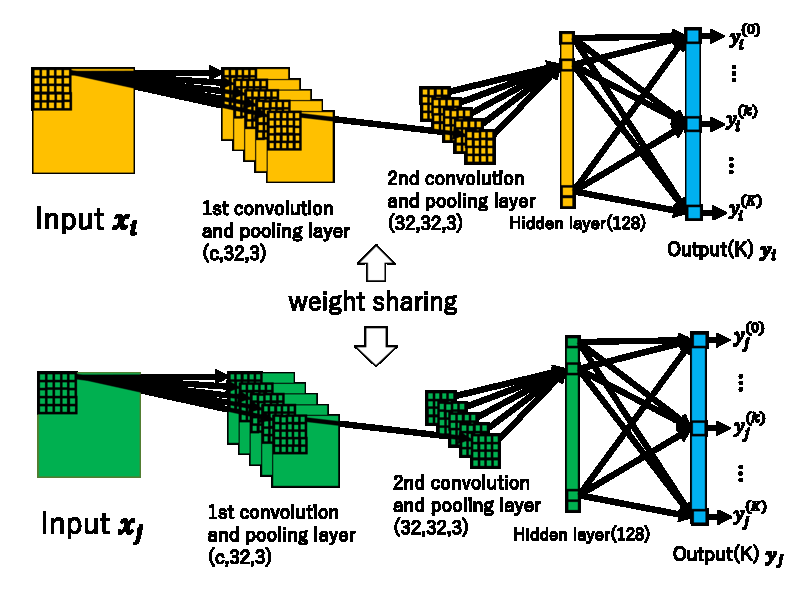
\includegraphics[width=100mm]{figure3.eps}
\caption{Siamese Network for multi-class classification}
\label{fig:siamese-mu}
\end{center}
\end{figure}
We extend the proposed binary classifier to multi-class classification by using one-vs-others approach.
%feature extractor in the binary classification proposed in the previous subsection to the multi-class feature extractor.
Figure \ref{fig:siamese-mu} shows the proposed Siamese Network for multi-class classification.
Similar with the Siamese Network for binary classification, the $K$ features $y^{(1)},y^{(2)},\ldots,y^{(K)}$ for $K$ classes classification are extracted by deep CNN.
%Each convolution layer and fully connected hidden layer are constructed in the same way as in the case of binary classification, and making the number of units of the output layer equal to the number of classes to be classified.

Each unit in the output layer of Siamese Network extracts a feature to classify the corresponding class and the other classes.
The constrastive loss of this network is defined as
%Each unit functions as a feature extractor such as in the case of a specific class and others classification. That is, considering the classification of $K$ classes now, labels are allocated to each unit, and contrastive loss is calculated for the output of each unit as shown in Equation (\ref{eq:multi contrastive}).
\begin{align} \label{eq:multi contrastive}
L_k&=\frac{1}{2|\chi^2|}\sum_{(i,j) \in \chi}^N l_{ij}^{(k)}(D^{(k)}_{ij})^2 + (1-l_{ij}^{(k)})max(m-D^{(k)}_{ij}, ~0)^2 \\
D^{(k)}_{ij}&=|y^{(k)}_{i}- y^{(k)}_{j}|^2
\end{align}
Where $\chi^2$ is an index set of sample pairs randomly generated from the mini-batch, $l^{(k)}_{ij}$ is a label in the binary classification when the $k$-th class is regarded as a positive class and the other classes are regarded as a negative class.
The distance $D^{(k)}_{ij}$ is defined as the distance between the pair of outputs $y_i^{(k)}$ and $y_j^{(k)}$ of the $k$-th unit.

The average of $K$ constrastive losses $L_k$  
\begin{align} \label{eq:ave contrastive}
E = \frac{1}{K}\sum_{k}^{K}L_k
\end{align}
is used to obtain the weights of the Siamese Network.
%Then, $k$-th unit of the output layer independently learns features for classifying the $k$-th class and others. \par

To estimate the posterior probability of each class from the features calculated by the Siamese Network, we use the multi-nominal logistic regression.
%Also in the case of multi-class classification, the problem of output described in the previous subsection occurs.
%Therefore, we extend the linear regression model described in the previous subsection for multi-class classification. \par
%In the case of multi-class classification, the number of output dimensions of siamese network is the number of classes to be classified.
The model of the multi-nominal logistic regression for the input vector $\bm{y}_n$ is given as
%So, the model of Equation (\ref{eq:regression}) is modified as follows.
\begin{align} \label{eq:regression multi}
    \hat{\bm y}_n = S(W\bm{y}_n+\bm{b})
\end{align}
where $W$ and $\bm{b}$ are the coefficient matrix and the bias vector respectively.
%Here, 
%\begin{align} \label{eq:string def}
%{\bm y}_n=\left[
%\begin{array}{c}
%y_n^{(0)} \\ 
%y_n^{(1)} \\
%\vdots \\
%y_n^{(K)}
%\end{array}
%\right], \hspace{0.2cm}
%W =\left[
%\begin{array}{ccc}
%w_{00} & \cdots & w_{0K} \\ 
%\vdots & \ddots & \vdots  \\
%w_{K0} & \cdots & w_{KK} \\
%\end{array}
%\right]
%\end{align} 
%Each element of ${\bm w}$ is an updatable weight and ${\bm b}$ is a bias. 
Also, $S(\cdot)$ is a softmax function (Equation(\ref{softmax})).
%In the case of multi class, the label ${\bm t}$ expresses which class a specific sample belongs with one-hot-vector.
Similar with the binary logistic regression, the log-likelihood for the training samples is defined as
\begin{align} \label{eq:multi crossentropy}
\hat{E} = \sum_n^N {\bm t}_n^Tlog(\hat{\bm y}_n) \; 
\end{align}
where $log(\hat{\bm y}_n)$ is the logarithm of each element of $\hat{\bm y}_n$. 
This is used to obtain the optimum parameters $W$ and $\bm{b}$ of the model.
It is known that this log-likelihood is the same as the cross entropy loss except the sign.
%\par
%As in the previous subsection, the optimum parameters ${\bm w}$ and ${\bm b}$ are obtained by maximizing this log-likelihood. \par

\subsection{Metric Learning for Knowledge Distillation}
\begin{figure}[ht]
\begin{center}
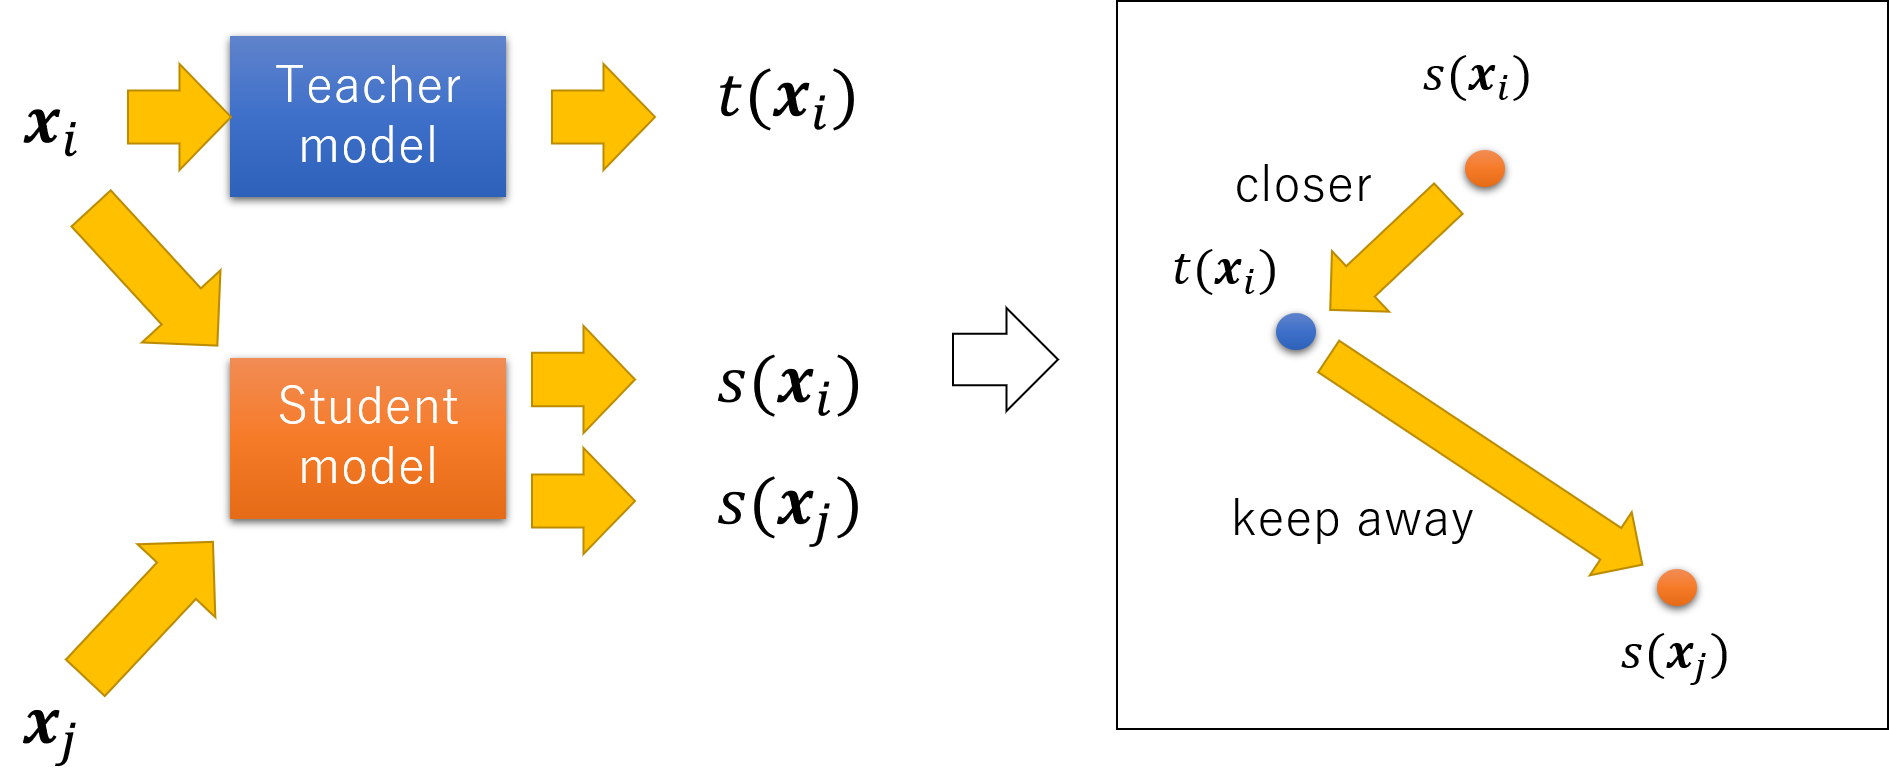
\includegraphics[width=80mm]{figure_ours.png}
\caption{The structure of our method. The student model is optimized so that its own output for sample $\bm{x}_a$ and the output of the teacher model for sample $\bm{x}_a$ are closer. At the same time, the student model is optimized so that its own output for sample $\bm{x}_n$ which is the different classes in the soft target and the output of the teacher model for sample $\bm{x}_a$ are keeping away.}
\label{fig:ours}
\end{center}
\end{figure}

Previously proposed methods of knowledge distillation focused on minimizing the difference between the teacher model and the student model in order to transfer knowledge of the teacher model.
For example,  Ba et al. \cite{Ba2014} considered the difference in model output as loss and Hinton et al. \cite{Hinton2015} considered the difference in model output distribution as loss.
In other words, they are solving the optimization problem in which the similarity between the function of the teacher model and the function of the student model is maximized.
There is a possibility that knowledge of the teacher model can be transferred to the student model by using the metric learning method to embed the neighboring relations of the teacher model in the output space of the student model.

Triplet \cite{Hoffer2015}, one of the deep metric learning methods, is a powerful method for learning similarity and dissimilarity (Equation (\ref{eq:triplet})).
Triplet loss has a function to reduce the output distance of "anchor-positive" and a function to increase the output distance of "anchor-negative".
We propose to apply this technique for knowledge distillation.

We define the triplet loss for knowledge transfer as
\begin{align}
    E_{ourKD} = \sum_{(a,n) \in \Omega} max(0, m + ||t({\bm x_a}) - s({\bm x_a})||_2^2 - ||t({\bm x_a}) - s({\bm x_n})||_2^2) \; ,
\end{align}
where $t(\cdot)$ is the output of the teacher model, $s(\cdot)$ is the output of the student model, and $m$ is the margin.
Further, ${\bm x_a}$ is a training sample extracted at random, and ${\bm x_n}$ is a sample classified into a different class from ${\bm x_a}$ in the case of a soft target.
$\Omega$ is the index set of each corresponding sample.
So, the output of the teacher model and the output of the student model for the same sample are considered as "anchor" and "positive", respectively.
Also we consider the output of the student model for samples of different classes in the case of soft target as "negative".
Since we are training the student model, the weight of the teacher model is not updated.
That is, $t(\cdot)$ is treated as a constant during training process.

For our loss, there is a term that makes the outputs of the teacher model and the student model closer. 
This is realized by making the square error of the outputs of the teacher model and the student model a loss.
This is similar to Ba et al. \cite{Ba2014} proposed function.
It is easy to define the loss by using KL-divergence similar with Hinton et al. \cite{Hinton2015}.
In addition, there are terms that increase the distance between outputs of different classes.
In other words, in addition to the conventional loss functions, it is possible to add a constraint that the student model makes the outputs of other classes dissimilar.
This will allow the student model to clarify differences in output between classes.
We have shown experimentally that this proposal contributed to the performance improvement of the student model.
We will also seek further performance improvements in combination with other distillation losses.

\section{Experiment}
In this section, we will experiment with the contributions of each of the efforts described in the previous section.
Each section describes the details of the experiment.
\subsection{Metric Learning for optimization of AUC}
In the experiment, we used Fashion-MNIST dataset and CIFAR-10 dataset.
Fashion-MNIST is a dataset in which grayscale images of 10 kinds of clothing items such as "trouser" and "dress" are included.
The image size is 28$\times$28, it has 6,000 train images per class and 1,000 test images per class.
CIFAR-10 is a dataset in which color images of 10 kinds of objects such as "automobile" and "dog" are included.
The image size is 32$\times$32, it has 5,000 train images per class and 1,000 test images per class.


At first, the effectiveness of the proposed approach for binary classification is investigated by comparing the proposed method with the standard CNN. Then the effectiveness for multi-class classification is investigated.
\subsubsection{Binary Classification}
At first we consider binary classification problems in which a specific target class and the other classes are classified.
Since there are ten classes in the datasets (Fashion-MNIST and CIFAR-10), we trained ten different networks for binary classification.
The Siamese Networks for binary classification shown in Figure \ref{fig:siamese-bi} are trained.
The experiment was performed changing the parameter $m$ in the loss of the Siamese Network in the range of 1 to 10.
It was found that the larger the $m$, the higher the score, but above 5 the learning becomes unstable.
Therefore, $m$ was set to 5.
The learning rate of SGD with momentum is initially set at 0.001 and divided by 10 every 100 epochs.
The momentum parameter is set to 0.9.
Then the parameters of the logistic regression model are determined to estimate the posterior probability of the target class.

For the comparison, the standard CNN with the same network structure with the Siamese Network is also trained as the baseline model.
The sigmoid function is used as the activation function of the output layer of the standard CNN and the binary cross entropy is used as the loss function.
AUC scores for the proposed model and the standard CNN are calculated.
For each model, the parameters of the networks are trained five times with different initial values and the average of the AUC scores are calculated for each target class.

The average AUC scores for Fashion-MNIST dataset are shown in Table \ref{tabel:AUC_Fashion_binary}.
Table \ref{table:AUC_CIFAR10_binary} shows the average AUC scores for CIFAR-10 dataset.
It is noticed that the average AUC scores of the proposed method are better than the standard CNN for many cases.
%The results show that in the binary classification of Fasion-MNIST and CIFAR10, the feature vector of siamese network improves the ROC-AUC score in many cases.
Especially for CIFAR-10 dataset almost all the average AUC scores of the proposed method are better than the standard CNN. 


%On the other hand, the baseline model, which is the object of comparison, consists of one network that outputs one value as shown in Figure 2.
%The sigmoid function is used as the activation function of the output layer, and the AUC is calculated from the output $y$ of the network. \par
%In the comparative experiment,  10-class datatset is used, and AUC scores of each model are compared by binary classification which classifies one specific classes (target class) and other classes.


%We consider binary classification which classifies a specific target class and other samples using the dataset mentioned above.
%We compare AUC of baseline model and AUC of siamese network when each class is taken as the target class.

%In addition, for each model, experiments are conducted with five kinds of initial weight values, and this average score is posted as a result. \par
%In order to prevent over learning, regularization term is added to loss as necessary.
%The AUC score in the binary classification that classifies the target class and the other classes is shown in the following Figure \ref{fig: binary auc fasion} and \ref{fig: binary auc cifar}.

For reference, Figure \ref{fig:roc-bi} shows the ROC curve for binary classification between "deer" and the other classes for CIFAR-10 dataset.
%For the class "coat" of fasion mnist dataset and the class "deer" of CIFAR10 dataset, the result of binary classification is shown by ROC curve (Figure \ref{fig:roc-bi}). \par
%It is noticed that the proposed method is better than the standard CNN classifier.

\begin{table}[ht]
\begin{center}
\caption{AUC of binary classification (Fasion-MNIST)}
\label{tabel:AUC_Fashion_binary}
\begin{tabular}{|c|c|c||c|c|c|} \hline
target class & Baseline & Siamese & target class &  Baseline & Siamese  \\ \hline \hline
class "t-shirt" &  ${\bf 0.9889}$       &     $0.9850$            &   class "sandal"        &  $0.9996$   &  ${\bf 0.9998}$   \\ \hline
class "trouser" &    $0.9992$   &         ${\bf 0.9999}$        &  class "shirt"          & ${\bf 0.9723}$   &   $0.9720$   \\ \hline
class "pullover" &    ${\bf 0.9891}$         &  $0.9854$               &  class "sneaker"          &  $0.9989$  &  ${\bf 0.9990}$    \\ \hline
class "dress" &   ${\bf 0.9955}$          &    $0.9928$            &     class "bag"      & $0.9985$       & ${\bf 0.9996}$ \\ \hline
class "coat" &   $0.9891$          &         ${\bf 0.9909}$       &    class "ankle boot"          & $0.9988$   & ${\bf0.9989}$    \\ \hline
\end{tabular}
\end{center}
\end{table}


\begin{table}[ht]
\begin{center}
\caption{AUC of binary classification (CIFAR-10)}
\label{table:AUC_CIFAR10_binary}
\begin{tabular}{|c|c|c||c|c|c|} \hline
class & Baseline & Siamese & class &  Baseline & Siamese  \\ \hline \hline
class "airplane" &     $0.9554$    &     ${\bf 0.9599}$          &   class "dog"        &$0.9292$     &  ${\bf 0.9323}$  \\ \hline
class "automobile" & $0.9783$      &    ${\bf 0.9827}$          &  class "frog"          & $0.9710$   &  ${\bf 0.9719}$    \\ \hline
class "bird" &     $0.9066$        & ${\bf 0.9076}$              &  class "horse"          & $0.9630$   & ${\bf 0.9653}$    \\ \hline
class "cat" &        ${\bf 0.8879}$     &    $0.8581$            &     class "ship"      &  $0.9771$      & ${\bf 0.9789}$ \\ \hline
class "deer" &     $0.9303$        &     ${\bf 0.9402}$           &    class "truck"          &  $0.9735$  & ${\bf 0.9785}$    \\ \hline
\end{tabular}
\end{center}
\end{table}
%\clearpage


\begin{figure}[ht] 
\centering
%\begin{tabular}{c}
%        \begin{minipage}{0.50\hsize}
%            \centering
%            \includegraphics[scale=0.4]{fasion_roccurve.png}
%        \end{minipage}
%          \begin{minipage}{0.50\hsize}
%            \centering
%            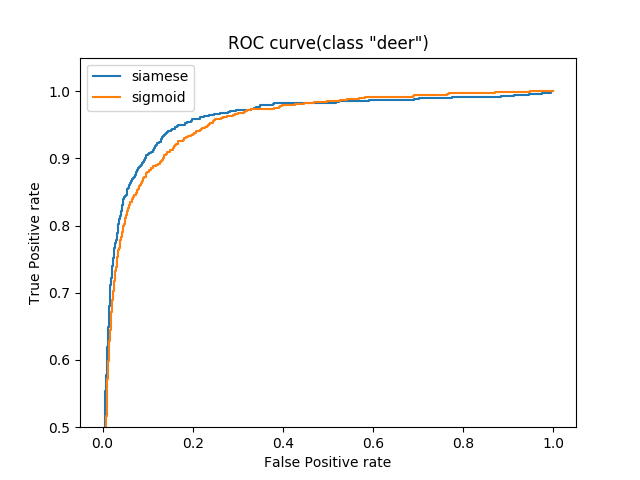
\includegraphics[scale=0.4]{roc_curve.png}
%        \end{minipage}
%\end{tabular}
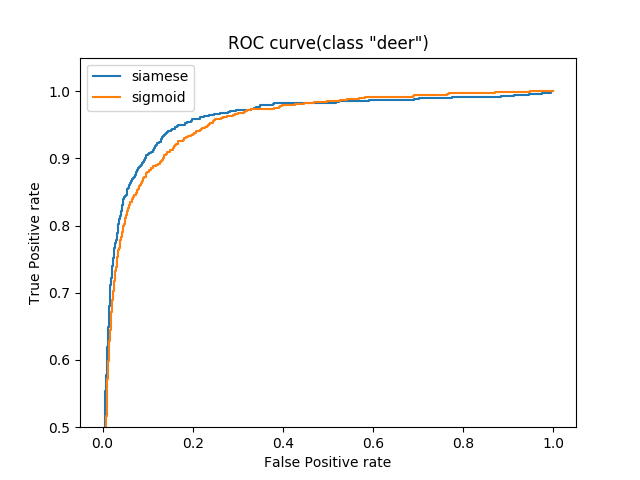
\includegraphics[scale=0.5]{roc_curve.png}
\caption{ROC curve for binary classification between "deer" and the other objects in CIFAR-10 dataset.}
\label{fig:roc-bi}
\end{figure}
\clearpage
\subsubsection{Multi-class Classification}
Here we investigate the effectiveness of the proposed method for multi-class classification.
The proposed model is trained by using Fashion-MNIST dataset and CIFAR-10 dataset.
The learning rate of SGD with momentum is initially set to 0.01 and divided by 10 at every 100 epochs.  
The  momentum parameter is set to  0.9. 
The parameter $m$ in the loss function of Siamese Network is set to 10.
As the baseline model, the standard CNN with softmax function as the activation function of the output layer is also trained to minimize the cross entropy loss.
Similar with the binary classification, the average AUC scores are measured for the proposed method and the standard CNN.
%For baseline model, learning of end to end is performed by crossentropy loss of Equation (\ref{eq:multi crossentropy}) using softmax function as the activation function of $K$ output layers.
%This is a general multi-class classifier model using a neural network. \par
%Comparison experiments compare the AUC scores of these two models.
The recognition accuracies for each model are also calculated.
%$\hat{\bm t}_n$ is a $K$-dimensional one-hot-vector with $\hat{y}_n^{(k)}$ as an element satisfying the following condition.
%\begin{align} \label{eq:accuracy}
%\hat{t}_n^{(k)}=\left\{
%\begin{array}{cc}
%1 & (k = argmax(y_n^{(0)}, y_n^{(1)}, \cdots, y_n^{(K)})) \\ 
%0 & (otherwise)
%\end{array}
%\right.
%\end{align} \par
In the case of multi-class classification, %each model is evaluated with accuracy and AUC.
we regard that each unit of the output layer solves the binary classification problem classifying the target class and the other classes and the average of the AUC scores of each output unit is calculated as the AUC score for each model.
%So, it is calculated AUC for each output unit.
%The average score of each calculated AUC is evaluated as the AUC score in the case of multi-class. 
For each model, the parameters of the networks are trained five times with different initial values and the average of the AUC scores are calculated.

The results are shown in Table \ref{table:AUC_ACC_multi}.
It is noticed that both of the average AUC score and the recognition accuracy of the proposed method is better than the standard CNN for multi-class classification.
%As a result of comparative experiments, also in the case of multi-class, improvement of AUC score was seen.
%And, siamese network exceeds the score in accuracy evaluation.
%By the way, in general crossentropy loss which uses sigmoid function as output activation function is used for binary classification using neural network.
%This sigmoid crossentropy considers positive and negative samples independently.
%On the other hand, the siamese network learns the metric between samples.
%As can be seen the figure, siamese network has higher accuracy and AUC score for both datasets.
Particularly in classification of CIFAR10, the recognition accuracy is about 3$\%$ better than the standard CNN.


ROC curves for CIFAR-10 dataset are shown in the Figure \ref{fig:roc-mul}. 
It is noticed that the proposed method gives better results than the standard CNN.

%In  addition,  for  each  model,  experiments  are conducted  with  five  kinds  of  initial  weight  values,  and  this average score is posted as a result. \par
%The accuracy and AUC for each dataset are shown in Table \ref{table:AUC_ACC_multi}.
%In  order  to  prevent  over  learning, regularization  term  is  added  to  loss  as  necessary.



\begin{table}[ht]
\begin{center}
\caption{AUC and accuracy for multi-class classification}
\label{table:AUC_ACC_multi}
\begin{tabular}{|c|c|c||c|c|c|} \hline
AUC & Baseline & Siamese & accuracy &  Baseline & Siamese  \\ \hline \hline
fasionMNIST & $0.9932$    & ${\bf 0.9941}$  &  fasionMNIST  & $0.9040$   &  ${\bf 0.9163}$ \\ \hline
CIFAR10  & $0.9601$      &  ${\bf 0.9635}$     &  CIFAR10   & $0.7219$     &${\bf 0.7538}$ \\ \hline
\end{tabular}
\end{center}
\end{table}
\clearpage

\begin{figure}[ht!]
\centering
%\begin{tabular}{c}
        %\begin{minipage}{0.50\hsize}
            \centering
            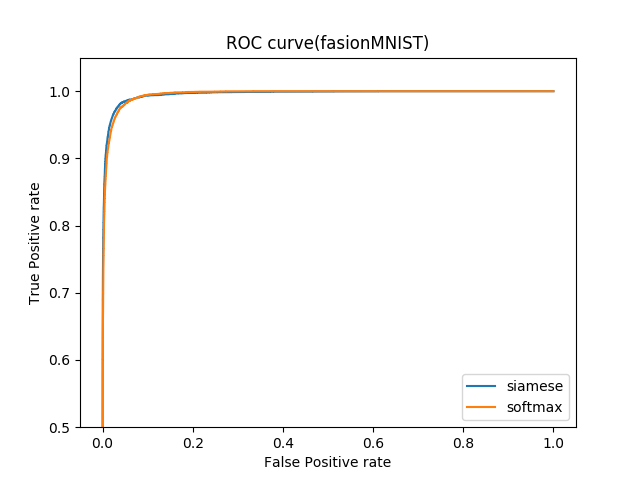
\includegraphics[scale=0.7]{fasion_multiroccurve.png}
           \\ (a) ROC curve for Fashion-MNIST dataset\\
        %\end{minipage}
          %\begin{minipage}{0.50\hsize}
            \centering
            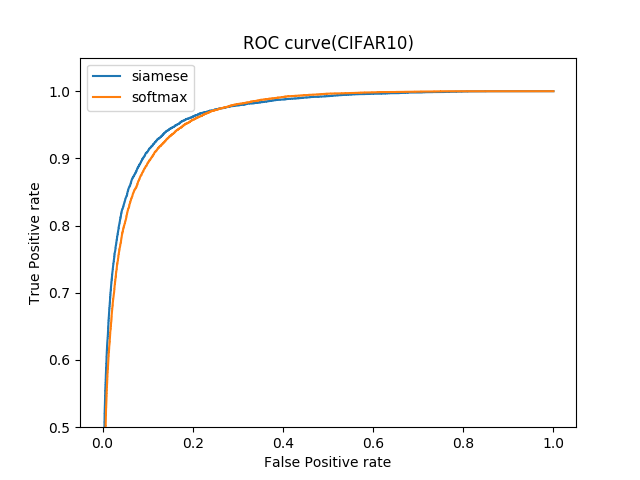
\includegraphics[scale=0.7]{multiroc_curve.png}
            \\ (b) ROC curve for CIFAR10 dataset\\
       % \end{minipage}
%\end{tabular}
\caption{ROC curve for multi-class classification}
\label{fig:roc-mul}
\end{figure}
%For both data sets, we can see that the proposed model depicts a slightly larger ROC curve.
%From the above, it can be seen that the feature vector of the siamese network contributes to increasing the ROC-AUC score.

\subsection{Metric Learning for Knowledge Distillation}
We experimentally investigated the effectiveness of the proposed method with the image classification task.
CIFAR-10 \cite{Krizhevsky2009} and Tiny ImageNet \cite{Le2015} are used as datasets.

\subsubsection{Experiments using CIFAR-10}

\begin{table}[ht] 
\caption{model structures for CIFAR-10}
\label{table:structure}
\begin{center}
\begin{tabular}{l|l} 
\hline
student model(5 layers) & teacher model(8 layers)   \\ \hline \hline
conv1(channel:32, filter:3) & conv1(channel:32, filter:3) \\
max pooling(2*2) & batch normalization(32) \\
conv2(channel:32, filter:3) & max pooling(2*2) \\
max pooling(2*2) & conv2(channel:32, filter:3) \\
conv3(channel:64, filter:3) & batch normalization(32) \\
max pooling(2*2) & max pooling(2*2) \\
fully-connected(128) & conv3(channel:64, filter:3) \\
output(10) & batch normalization(64) \\
 & conv4(channel:64, filter:3) \\
 & batch normalization(64) \\
 & conv5(channel:128, filter:3) \\
 &  batch normalization(128) \\
 & max pooling(2*2) \\
 & fully-connected(512) \\
 & dropout \\
 & fully-connected(128) \\
 & dropout \\
 & output(10) \\
\hline
\end{tabular}
\end{center}
\end{table}

CIFAR-10 is a dataset that includes color images of 10 kinds of objects such as "automobile" and "dog."
The size of each image in CIFAR-10 is $32 \times 32$.
The numbers of the training samples and the test samples are 50,000 and 10,000.
We conducted comparative experiments with Ba's KD \cite{Ba2014} (BKD), Hinton's KD \cite{Hinton2015} (HKD), and Park's RKD-DA \cite{Park2019}.

In the case of CIFAR-10, the 8-layers CNN model shown in Table \ref{table:structure} was used as a teacher model, and the 5-layers CNN model was used as a student model.
The number of trainable parameters of the student model is 161,130, and the number of trainable parameters of the teacher model is 1,256,106. 
The number of parameters in the student model is about 12.8$\%$ of the number of parameters in the teacher model.

An activation function ReLU defined by
\begin{align} \label{eq:ReLU}
h(x) = max(0,x)
\end{align}
is used for the outputs of each convolution layer and the outputs of each fully-connected layer except for the last output layer.

In the training, the optimization is done by using the stochastic gradient descent (SGD) with momentum.
The learning rate of SGD is initially set at 0.01 and changed by multiplying 0.1 at every 100 epochs. 
The momentum parameter is set to 0.9.
We also introduced weight decay to prevent over-learning.
We set hard target loss as cross entropy with softmax and combined it with soft target loss.
In addition, we introduced a parameter $\lambda$ as shown in Equation (\ref{eq:distillation loss}) to maintain the balance between hard target loss and soft target loss.
We set $\lambda_{BKD}=2$, $\lambda_{HKD}=16$, $\lambda_{RKD-D}=10$, $\lambda_{RKD-A}=20$ and $\lambda_{oursKD}=2$.
The temperature parameter of Hinton's KD \cite{Hinton2015} was set to 4, and the hyper-parameter $m$ of triplet loss was set to 5.


\begin{table}[ht]
\caption{Classification accuracy for CIFAR-10}
\label{table:cifar-10}
\begin{center}
\begin{tabular}{|l|l|}
\hline
method & accuracy \\ \hline \hline
Student model & $74.66\%$ \\ \hline
Ba's KD & $80.40\%$ \\ \hline
Hinton's KD & $79.16\%$ \\ \hline
RKD-DA &       $79.21\%$     \\ \hline
Ours KD & $\bm{81.14}\%$ \\ \hline \hline
Teacher model  & $83.42\%$     \\
\hline
\end{tabular}
\end{center}
\end{table}

The Table \ref{table:cifar-10} shows the classification accuracy of the student model for test samples in each method.
From the table, it can be seen that in the case of CIFAR10, the proposed method achieves higher performance than the other methods.


\subsubsection{Experiments using Tiny ImageNet}

Also, we have performed experiments using the Tiny ImageNet dataset.
Tiny ImageNet dataset includes color images of 200 kinds of objects.
The image size is $64 \times 64$, and it has 500 train images and 50 test images per class.
For the case of Tiny ImageNet, VGG19 with batch normalization and VGG11 were used as the teacher model and the student model, respectively.
The numbers of trainable parameters of the teacher model and the student model are 46,028,808 and 35,213,896, respectively.
This means that the number of parameters of the student model is about 76.5$\%$ of those of the teacher model.
We conducted comparative experiments with Ba's KD \cite{Ba2014} (BKD), Hinton's KD \cite{Hinton2015} (HKD), and Park's RKD-DA \cite{Park2019}.


The weights in the convolution layers were pre-trained by using ImageNet, and they were used as the initial weights of the training.
Similarly, the SGD with momentum was used for the optimization.
The learning  rate  of  SGD  with momentum is initially set at 0.001 and multiplied by 0.9  every 3 epochs.  
The  momentum parameter  is  set  to  0.9. 
We also used mixup \cite{Zhang2017} to prevent over-learning.
 Cross-entropy with softmax was used as the hard target loss and was combined with the soft target loss.
Also, we introduced a parameter $\lambda$ as shown in Equation (\ref{eq:distillation loss}) to maintain the balance between hard target loss and soft target loss.
We set $\lambda_{BKD}=2$, $\lambda_{HKD}=16$, $\lambda_{RKD-D}=25$, $\lambda_{RKD-A}=50$ and $\lambda_{oursKD}=2$.
The temperature parameter of Hinton's KD \cite{Hinton2015} was set to 4, and the parameter m of triplet loss was set to 5.


\begin{table}[ht]
\caption{Classification accuracy for Tiny ImageNet}
\label{table:imagenet}
\begin{center}
\begin{tabular}{|l|c|}
\hline
method & accuracy \\ \hline \hline
Student model & $58.63\%$ \\ \hline
Ba's KD & $59.80\%$ \\ \hline
Hinton's KD & $59.80\%$ \\ \hline
RKD-DA & $59.73\%$     \\ \hline
Ours KD & $\bm{60.00}\%$ \\ \hline \hline
Teacher model  & $63.17\%$    \\
\hline
\end{tabular}
\end{center}
\end{table}

Table \ref{table:imagenet} shows the classification accuracy of the student model for the Tiny ImageNet dataset in each method.
The results show that the proposed method gives slightly better performance than the other methods.


\subsubsection{Experiments on the combined loss}

Park et al. \cite{Park2019} succeeded in achieving even higher performance by combining their method (RKD-DA) with Hinton's method \cite{Hinton2015}.
Here we investigate the effectiveness of the combination of different loss functions.
The loss of each method is combined with Hinton's loss as
\begin{align} \label{eq:distillation loss2}
E = E_{hard} + \lambda_{soft} E_{soft} + \lambda_{HKD} E_{HKD}
\end{align}.
Depending on the datasets CIFAR-10 and Tiny ImageNet, the same network architectures with the previous subsections were used.
The student models were trained, and the classification performances of the trained student models are calculated.

\begin{table}[ht]
\caption{Classification accuracy for combined with HKD}
\label{table:combined}
\begin{center}
\begin{tabular}{|l|c|c|}
\hline
method & CIFAR10 & Tiny ImageNet \\ \hline \hline
Student model &$74.66\%$  & $58.63\%$ \\ \hline
Hinton's KD & $79.16\%$ & $59.80\%$  \\ \hline
Ba's KD + HKD & $80.33\%$ & $60.19\%$  \\ \hline
RKD-DA + HKD &  $79.65\%$   & $59.89\%$      \\ \hline
Ours KD + HKD & $\bm{80.93}\%$ & $\bm{60.62}\%$  \\ \hline \hline
Teacher model  & $83.42\%$  & $63.17\%$  \\
\hline
\end{tabular}
\end{center}
\end{table}

Table \ref{table:combined} shows the classification performance of the test samples for each dataset.
From this table \ref{table:combined}, it is noticed that the classification accuracy of Park's KD \cite{Park2019} was improved by combining with the Hinton's loss for CIFAR-10 dataset, but the classification accuracy of the proposed method and Ba's KD \cite{Ba2014} was not improved.
However the proposed method still gives the best classification accuracy.
For the Tiny ImageNet dataset, all methods showed an increase in the classification accuracy when they are combined with Hinton's KD \cite{Hinton2015}.
Also, the proposed method gives the best accuracy for this case.

Also we consider a combination with Park's KD \cite{Park2019}.
We investigate the effects of combining RKD-DA loss with our loss and we investigate combinations with both Hinton's KD \cite{Hinton2015} and RKD-DA.
Depending on the datasets CIFAR-10 and Tiny ImageNet, the same network architectures with the previous subsections were used.

\begin{table}[ht]
\caption{Classification accuracy of ours KD for combined with RKD-DA}
\label{table:combinedRKD}
\begin{center}
\begin{tabular}{|l|c|c|}
\hline
method & CIFAR10 & Tiny ImageNet \\ \hline \hline
Student model &$74.66\%$  & $58.63\%$ \\ \hline
RKD-DA & $79.21\%$  & $59.73\%$   \\ \hline
ours KD & $\bm{81.14}\%$ & $60.00\%$   \\ \hline
ours KD + RKD-DA & $80.17\%$    &  $\bm{60.32}\%$     \\ \hline
ours KD + HKD + RKD-DA &  $80.30\%$   & $\bm{60.65}\%$      \\ \hline
Teacher model  & $83.42\%$  & $63.17\%$  \\
\hline
\end{tabular}
\end{center}
\end{table}

Table \ref{table:combinedRKD} shows the classification accuracy of the student model in each method.
In the case of the CIFAR10 dataset, no performance improvement was obtained even when combined with RKD-DA.
In the case of the Tiny ImageNet dataset, we succeeded in improving performance by combining it with RKD-DA.
In addition, using both RKD-DA and Hinton's KD in combination with our method resulted in further performance improvements.
Although the combination of our method and Hinton's KD had improved the performance, the combination of both Hinton's KD and RKD-DA achieved even higher performance.
\section{Conclusion}
\bibliographystyle{unsrt}
\bibliography{reference.bib}
\end{document}
